\Chapter{Capturing A Shape-Shifter: The Semantic Process}{A Formal Foundation for Strategic Rewriting}
\label{chap4}

\begin{tikzpicture}[color=black,
                   transform shape,
                   every node/.style={inner sep=0pt}]
% \node[minimum size=\framesize,fill=white](vecbox){};
% \node[text width=\framesize,align=center](Text){%
%     `Then you should encode what you mean', the March Hare went on.
% \\
% `I do', Programmer hastily replied; `at least --- at least I mean what I encode --- that's the same thing, you know.'
% \\
% `Not the same thing a bit', said the Hatter.};
\node[minimum width=\framesize, minimum height=0.55 *\framesize, fill=white](vecbox){};
\node[anchor=north west] at (vecbox.north west){% 
\pgfornament[width=0.1*\framesize]{61}};
\node[anchor=north east] at (vecbox.north east){% 
\pgfornament[width=0.1*\framesize,symmetry=v]{61}};
\node[anchor=south west] at (vecbox.south west){% 
\pgfornament[width=0.1*\framesize,symmetry=h]{61}};
\node[anchor=south east] at (vecbox.south east){% 
\pgfornament[width=0.1*\framesize,symmetry=c]{61}};
\node[anchor=north] at (vecbox.north){% 
\pgfornament[width=0.25*\framesize]{88}
% \pgfornament[width=0.1*\framesize]{15}
% \pgfornament[width=0.1*\framesize]{16}
\pgfornament[width=0.25*\framesize]{88}
\pgfornament[width=0.25*\framesize]{88}
};

\node[anchor=south] at (vecbox.south){% 
% \pgfornament[width=0.25*\framesize]{88}
% \pgfornament[width=0.1*\framesize,symmetry=h]{15}
\pgfornament[width=0.25*\framesize]{88}
\pgfornament[width=0.25*\framesize]{88}
\pgfornament[width=0.25*\framesize]{88}
% \pgfornament[width=0.1*\framesize,symmetry=h]{16}
% \pgfornament[width=0.25*\framesize]{88}
};
% \node[anchor=south] at (vecbox.south){% 
% \pgfornament[width=0.6*\framesize]{46}};
% \node[anchor=north,rotate=90] at (vecbox.west){% 
% \pgfornament[width=0.6*\framesize,symmetry=h]{46}};
% \node[anchor=north,rotate=-90] at (vecbox.east){% 
% \pgfornament[width=0.6*\framesize,symmetry=h]{46}};
\node[text width=0.85\framesize,align=justify] at (vecbox.center){%
It was a terrible, indescribable thing vaster than any subway train—a shapeless congeries of protoplasmic bubbles, faintly self-luminous, and with myriads of temporary eyes forming and unforming as pustules of greenish light all over the tunnel-filling front that bore down upon us \dots 
%crushing the frantic penguins and slithering over the glistening floor that it and its kind had swept so evilly free of all litter. Still came that eldritch, mocking cry --- \textit{``Tekeli-li! Tekeli-li!"} 
And at last we remembered that the daemoniac \emph{shoggoths} --- given life, thought, and plastic organ patterns solely by the Old Ones, and having no language save that which the dot-groups expressed --- had likewise no voice save the imitated accents of their bygone masters.\\
\rightline{--- H. P. Lovecraft ``From the Mountains of Madness"}};
% \node[text width=0.85\framesize,align=right] at (vecbox.south){%
%    --- \emph{Altered} Alice's Adventures in Wonderland};
\end{tikzpicture}
\noindent
\begin{center}
\vspace{0.3em}
\begin{tikzpicture}[color=black,
                   transform shape,
                   every node/.style={inner sep=0pt}]
\node[minimum width=0.35\framesize, minimum height=0.05*\framesize, fill=white](vecbox){};
\node[anchor=west] at (vecbox.west){\pgfornament[width=0.08*\framesize]{16}};
\node[anchor=east] at (vecbox.east){\pgfornament[width=0.08*\framesize]{15}};
\node[inner sep=6pt] (text) at (vecbox.center){\textbf{\Large Prologue}};
\end{tikzpicture}
\vspace{-0.7em}
\end{center}
% \section{Prologue}
% \label{chap4:prologue}
\lettrine{S}{hoggoth}, as illustrated in the quotation, is a Lovecraftian \emph{shape-shifting monster}, making the sound ``Tekeli-li, Tekeli-li" which can no longer be understood by anyone. In this chapter, we thoroughly discuss a foundational study of a domain specific programming language --- a strategic rewriting language for \emph{syntactic transformations}, which previously lacked a formal treatment. By making a metaphorical connection, we named the study Shoggoth and published it under the title \emph{Shoggoth: A Formal Foundation for Strategic Rewriting}.

In chapter~\ref{chap1}, we briefly discussed that conceptually it is intriguing to explore the relationship between syntax and semantics within the context of strategic rewriting. Since term rewriting, as a technique of syntactic transformations, encodes the semantics of some programs, and compositions of each individual term rewriting step form strategies, of which the straightforward syntax is given by a strategic rewriting language, whose semantics featuring non-termination and non-deterministic executions is complicated and worth studying to allow us to formally understand and reason about the composition of these rewrites.

In this chapter, we utilise three formal semantics models of programming languages, namely, denotational semantics, big-step operational semantics, and axiomatic semantics, to analyse a core calculus of a set of strategic rewriting languages, and discuss how these models relate to each other.

\section{Introduction}
\label{chap4:introduction}
Strategic rewriting allows programmers to compose rewrite rules and control their application.
Dedicated strategy languages, such as Stratego~\citep{DBLP:conf/icfp/VisserBT98,10.1007/3-540-45127-7_27} and more recently Elevate~\citep{DBLP:journals/cacm/HagedornLKQGS23,DBLP:journals/pacmpl/HagedornLKQGS20}, provide combinators for composing rewrite rules into larger strategies, as well as traversals to describe the location at which rewrite strategies are applied.

Strategic rewriting has many important practical applications. For instance, Stratego is used to specify the semantics of programming languages by writing interpreters with rewrite strategies in the Spoofax language workbench~\citep{DBLP:journals/software/WachsmuthKV14}.
Elevate is used to describe compiler optimisations for generating fast code achieving competitive performance to the state-of-the art machine learning compiler TVM~\citep{DBLP:journals/pacmpl/HagedornLKQGS20}. Strategic rewriting is also used in domains ranging from generic programming~\citep{DBLP:conf/rule/LammelV02} to tactic languages in proof assistants~\citep{sozeau2014proof}.

\begin{highlightnew}
To give some examples of strategic rewriting, rewrite rules like $\mathit{add_{id}}$ and $\mathit{add_{com}}$ shown below are what we call \emph{atomic strategies}:
\[\mathit{add_{id}} : 0 + a \rightsquigarrow a \quad\quad\quad\mathit{add_{com}}: a + b \rightsquigarrow b + a\]
These two strategies can be composed into a new strategy using a sequential composition \emph{combinator} ($\seqcomp$), such a composed strategy is shown below:
\[\mathit{add_{com}}\seqcomp\mathit{add_{id}}\]
This strategy instructs to execute the atomic strategy $\mathit{add_{id}}$ after the execution of the atomic strategy $\mathit{add_{com}}$. It can rewrite an expression $3+0$ into $3$. We introduce the formal syntax of strategies together with more examples in section~\ref{chap4:syntax}.
\end{highlightnew}

Compositions of rewrites easily become complex.
For example, \citet{DBLP:journals/pacmpl/HagedornLKQGS20} report that for performing their compiler optimisations up to $60,000$ rewrite steps are required. To orchestrate such long rewrite sequences, strategy languages provide various combinators for composing strategies together and traversals for applying strategies to different sub-expressions within the given abstract syntax tree.
Together with support for recursion, these combinators and traversals are capable of modelling the complex rewrite sequences required in practical applications.

This capability comes at the cost of semantic complexity, as strategies can be nondeterministic, they may give an error which triggers backtracking, and they may diverge due to the presence of general recursion. Such a combination of features introduces a lot of semantic subtleties, which make it
easy to define not well-behaved strategies by mistake. For example, a strategy that does not terminate as it repeatedly tries to apply a rewrite.
Similarly, it is easy to compose incompatible rewrites
that will fail for every possible input expression.
Finally, even if a rewrite strategy successfully terminates, it may not do what it was supposed to do by rewriting the input expression into an undesired form.

The goal of this chapter is to provide a rigorous treatment of strategic rewriting, that we believe lacks so far. Considering that strategic rewriting has various application domains but has problematic behaviours, a rigorous formal understanding of strategic rewriting is required to model and analyse its semantic subtleties as well as reason about the execution of strategies. Therefore, we present Shoggoth: a formal foundation for reasoning about strategic rewriting.

We start with introducing the formal syntax of \emph{System S}, a formal core strategy language
originally introduced by \citet{VISSER1998422}. Some example strategies are sketched to give the gist of strategic rewriting as well. We then give a comprehensive semantic
accounting of strategic rewriting languages. We define a \emph{denotational semantics} for System
S, which originally had been given
a \emph{big-step operational semantics}. Our denotational semantics accounts for non-determinism and errors, and, unlike previous work, also explicitly models divergence.
In addition, we formalise an extended big-step operational semantics which accounts for diverging executions, and formally prove the equivalence of our two models via soundness and computational adequacy theorems. All of our results have been mechanised in Isabelle/HOL~\citep{NipkowPauWen:IsabelleTut:2002}.

To facilitate formal reasoning about rewriting strategies, we define a \emph{weakest precondition calculus} that for a given postcondition computes the weakest precondition that must hold in order for the given strategy to execute successfully and satisfy the postcondition. Because traversals allow us to apply strategies to sub-expressions of the input expression, we must know not just which rewrite rules are to be applied, but also \emph{where} in the input expression they are to be applied, in order to determine the weakest precondition. To accomplish this, our weakest precondition calculus is \emph{location-based}: weakest preconditions are not just based on the given strategy and desired postcondition, but also depend on the location at which the strategy is to be applied in the input expression. We have mechanised the definition of the weakest precondition calculus in Isabelle/HOL and formally proven its soundness with respect to the denotational semantics. 

Finally, we show how to use the weakest precondition calculus to reason about rewrite strategies by applying it to various examples, including termination, that a strategy is well-composed, and that a rewrite strategy satisfies a particular postcondition after its execution.
One of our examples is a strategy for $\beta\eta$-normalisation taken from the Elevate project by \citet{DBLP:journals/pacmpl/HagedornLKQGS20}, demonstrating the applicability of our work to practical scenarios.

In summary, we make the following contributions:
\begin{itemize}
  \setlength\itemsep{1.6ex}
    \item We design, formalise and mechanise using Isabelle/HOL the semantics of System S, including both denotational and operational models with a full accounting of nondeterminism, errors, and divergence. We prove these two semantics equivalent (Section~\ref{chap4:semantics}).
    \item We design, formalise and mechanise using Isabelle/HOL a location-based weakest precondition calculus for System S. We prove its soundness with respect to the denotational semantics (Section~\ref{chap4:wp}).
    \item We demonstrate how to use the weakest precondition calculus to prove practical useful properties of strategic rewriting (Section~\ref{chap4:reasoning}):
    \begin{itemize}
    \setlength\itemsep{0ex}
        \item that a strategy terminates, i.e., that is does not diverge;
        \item that a strategy is well-composed, i.e., that there exist input expressions for which the strategy execution will succeed;
        \item that a desired property is satisfied after execution of the strategy.
    \end{itemize}
\end{itemize}

Before stepping into the formalisation of System S, in the next section we present the syntax of System S as well as some example strategies to facilitate the understanding of strategic rewriting.

\section{The Syntax of System S}
\label{chap4:syntax}
System S \citep{VISSER1998422} is a core
calculus providing basic constructs of strategic rewriting,
including atomic strategies (rewrite rules) and operators
composing strategies and performing expression traversals in an abstract syntax tree (AST). A
successful execution of a strategy transforms an expression into some other expression while
preserving its semantics. The expressions being rewritten can either be $\mathit{Leaf}$s or $\mathit{n}$odes, in general, taking the form of:
\begin{alignat*}{3}
\mathrm{Expression} (\mathbb{E}) \quad
&e \ &\metaDeff \quad &\mathit{Leaf} \cmid\begin{array}{@{}c@{}} \begin{tikzpicture}[level distance=1.5em] \Tree [ .$\mathit{n}$ $e$ $e$ ]\end{tikzpicture}\end{array}
\end{alignat*}

Figure~\ref{chap4:syntax:syntax} presents the syntax of strategies in System S. We use $\mathbb{S}$ to denote the set of all strategies. Variables, atomic strategies, \sskip and \sabort are \textit{basic strategies}. Basic strategies are not decomposable. An atomic strategy is simply a rewrite rule. For instance, the commutativity of addition $\mathit{add_{com}}$ and commutativity of multiplication $\mathit{mult_{com}}$ are atomic strategies:
\begin{align*}
    &\mathit{add_{com}}: a + b \rightsquigarrow b + a &\text{Commutativity of addition}\\
    &\mathit{mult_{com}}: a * b \rightsquigarrow b * a &\text{Commutativity of multiplication}
\end{align*}
$\sskip$ can always be executed successfully while executing $\sabort$ would always cause failure. To compose strategies, one can make use of \textit{combinators} including sequential composition ($\seqcomp$), left choice ($\lchoice$) and nondeterministic choice ($\choice$). Sequential composition instructs to execute two strategies one after the other. Left choice prefers executing the strategy at the left hand side of the combinator over the strategy at the right hand side of the operator while nondeterministic choice decides to execute one of the given two strategy nondeterministically. In addition, $\one$, $\some$ and $\all$ are \textit{traversals} that navigate within the AST. Intuitively, $\one(s)$ applies $s$ to one immediate sub-expression of an input expression, $\some(s)$ applies $s$ to as many immediate sub-expressions of an input expression as possible and   $\all(s)$ applies $s$ to all immediate sub-expressions of an input expression. Lastly, System S provides a \textit{fixed-point operator} to model recursion.
\begin{figure}
\begin{alignat*}{3}
    \text{Strategy}(\mathbb{S}) \quad
    s \ \metaDeff &\ \mathit{atomic}
    \cmid X \cmid \sskip \cmid \sabort
    \\ \cmid &s\seqcomp s
    \cmid s \lchoice s
    \cmid s \choice s
    \\ \cmid &\one(s)
    \cmid \some(s)
    \cmid \all(s)
    \\ \cmid &\mu X. s
\end{alignat*}
\caption{The Syntax of System S}
\label{chap4:syntax:syntax}
\end{figure}
\paragraph*{Comparison of the expressiveness to the original System S}One difference between our formalism and the original System S is that we abstract away the term building details for atomic strategies, instead modelling atomic strategies as partial functions. We believe that applying this abstraction does not limit the expressiveness of our system. In fact, the purpose of such design is to allow the flexibility of the term languages, not only limited to the original System S, but also capturing other strategic rewriting languages that use term constructs that are different from System S. Moreover, this design enables us to focus on reasoning about properties of compositions of rewriting strategies that hold independent of the term building behaviour.

\paragraph*{Composing strategies}We can compose strategies together with these combinators, traversals and the fixed-point operator to define more strategies. For example, we define a strategy $\try(s)$ using left choice and \sskip which attempts to apply a strategy $s$ to an input expression. If an error occurs, then it will leave the input expression unchanged by executing the strategy \sskip:
\[\try(s) \metaDef s \lchoice \sskip\]
With the fixed-point operator and sequential composition, we can then define a strategy $\mathit{repeat}(s)$ which keeps applying a strategy $s$ to an input expression until its no longer applicable:
\[\mathit{repeat}(s) \metaDef \mu X. \mathit{try}(s\seqcomp X)\]
With the fixed-point operator, the traversal $\mathit{one}(s)$ and left choice, we can define top-down and bottom-up traversals in an AST:
\begin{align*}
    &\mathit{topDown} (s) \metaDef \mu X. (s \lchoice \one(X))
    &\mathit{bottomUp} (s) \metaDef \mu X. (\one(X) \lchoice s)
\end{align*}
We can further compose $\mathit{repeat}(s)$ and $\mathit{topDown}(s)$ to define a strategy $\mathit{normalise}(s)$, which keeps applying a strategy $s$ to all sub-expressions of an input expression until it is no longer applicable:
\[\mathit{normalise} (s) \metaDef \mathit{repeat}(\mathit{topDown}(s))\]
The $\mathit{normalise}$ strategy is very commonly used for expressing program transformations. Given $\mathit{beta}$ and $\mathit{eta}$ reductions for $\lambda$-expressions, we can use the normalisation strategy $\mathit{normalise}(\mathit{beta} \lchoice \mathit{eta})$ for normalising an input $\lambda$-expression into its $\beta\eta$-normal form.

As previously mentioned, the composition of strategies can be invalid and the executions of strategies are not always successful. For instance, the strategy $\mathit{mult_{com}}\seqcomp\mathit{add_{com}}$ is not well composed since it cannot be successfully executed on any input expression. $\mathit{repeat}(\sskip)$ is a strategy that cannot terminate. Although $\mathit{normalise}(\mathit{beta} \lchoice \mathit{eta})$ can certainly be successfully executed on some input expressions, on other inputs it may not terminate. It is important to know that when it terminates, it will indeed leave the expression in $\beta\eta$-normal form.

To reason about the successful and unsuccessful executions of strategies, we design the \emph{location-based weakest precondition calculus} which is discussed in section~\ref{chap4:wp}. With this calculus, we are able to detect \emph{bad} strategies that do not have successful executions, like $\mathit{mult_{com}}\seqcomp\mathit{add_{com}}$ and $\mathit{repeat}(\sskip)$, by concluding that there is no input expression that can be successfully rewritten by such strategies into a desired form. Also, for a \emph{good} strategy that has successful executions, we are able to distinguish inputs that indeed lead to successful executions of the strategy and inputs that lead to erroneous or diverging executions. Such reasoning power is demonstrated in section~\ref{chap4:reasoning}.  

To design the location-based weakest precondition calculus, we need to understand the behaviours of executing these strategies in System S. Therefore, before introducing the calculus and its reasoning power, we firstly study the formal semantics of System S.

\section{The Semantics of System S}
\label{chap4:semantics}
For given collections of expressions $\mathbb{E}$, System S defines nondeterministic executions for given strategies that can result in expressions or errors. We extend the original System S by allowing divergence as a possible result of executing a strategy. Thus, applying a strategy to an expression can result in expressions, an error or divergence.

\subsection{The Plotkin Powerdomain}
\label{chap4:subsec:plotkin}
We provide a denotational semantics of System S as an instance of Plotkin's powerdomain construction
\citep{plotkin:powerdomain}, which allows us to assign least fixed points as the semantics of the
recursion construct. An \emph{$\omega$-complete partial order} (\emph{$\omega$-cpo}) is a partially
ordered set $(X,\preceq)$ in which each $\omega$-chain ($x_1 \preceq x_2 \preceq x_3 \preceq \dots$)
has a least upper bound. A function $f:X \rightarrow X$ on such a set is \emph{continuous} if for
each $\omega$-chain $x_1 \preceq x_2 \preceq x_3 \preceq \dots$ with least upper bound $x$, one has
that $f(x)$ is the least upper bound of the set $\{f(x_1),f(x_2),f(x_3),\dots\}$.
A continuous function is certainly \emph{monotone}, in the sense that $x_1 \preceq x_2$ implies
$f(x_1) \preceq f(x_2)$ -- this follows by considering the $\omega$-chain
$x_1 \preceq x_2 \preceq x_2 \preceq x_2 \preceq \dots$, and its least upper bound $x_2$.
Now Kleene's fixed-point theorem says that each continuous function $f$ on an $\omega$-cpo with a least
element has a least fixed point.

Consider a nondeterministic, possibly diverging, algorithm that transforms values into values.
If $\V$ is the set of values, this algorithm can be modelled as a function
$f:\V \rightarrow \Pow_{\neg \emptyset}(\V_\bot)$, where
$\Pow_{\neg \emptyset}(X)$ is the set of non-empty subsets of $X$, the non-empty-powerset, and
$\V_\bot:= \V \uplus \{\bot\}$ is the set in which we embed $\V$ together with a new element $\bot$. The newly added element $\bot$ represents
the outcome where the algorithm diverges.
We equip the set $\V_\bot$ with a partial order by defining:
\[x \preceq y \iff x = \bot \lor x = y\;.\]
This fits with the intuition that $\bot$ represents a computation that has not yet
terminated, and $x \preceq y$ holds when $y$ is a later stage of the computation $x$.\\

Terminated computations are identified by the values they compute. We compare
sets of values using the Egli-Milner ordering:\vspace{1ex}\\
\( A \preceq B 
\iff (\forall x \in A.\; \exists y \in B.\; x \preceq y) \land (\forall y \in
B.\; \exists x \in A.\; x \preceq y)\)\vspace{1ex}

\begin{wrapfigure}{r}{0.35\textwidth}
  \vspace{-25pt}
  \begin{center}
    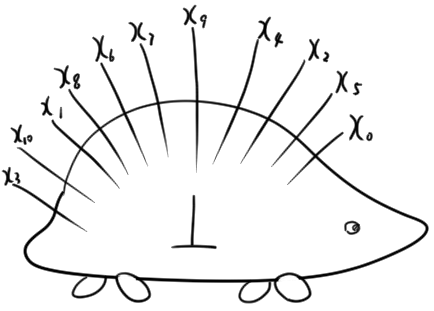
\includegraphics[width=0.3\textwidth]{porcupine.png}
  \end{center}
\end{wrapfigure}%

\noindent Lifting a partial order from elements to sets in this
fashion always yields a preorder. For a \emph{flat domain} $\V_\bot$, $\preceq$ is a partial order on
$\Pow_{\neg \emptyset}(\V_\bot)$. It is characterised by:
\begin{align*}
     &A \preceq B \iff  A = B \lor ((\bot \in A) \land A {\setminus} \{\bot\} \subseteq B)  &\qquad\qquad\quad\text{\centering(Porcupine ordering)}
\end{align*}
The resulting poset $\Pow_{\neg \emptyset}(\V_\bot)$ is an $\omega$-cpo.
Each $\omega$-chain either enters a spine of the
porcupine, and thus contains a largest element which is its least upper bound,
or $\bot$ is a member of all elements in the chain, so that its least upper bound is simply the union of all sets in the chain.

\paragraph*{Aside on the powerdomain construction and the Egli-Milner ordering.}
To give some further insight into the powerdomain construction and the Egli-Milner ordering, recall the following well-known characterisation. \citet[Remark after Lemma~3.5]{hennessy-plotkin:plotkin-powerdomain} show that
\citepos{plotkin:powerdomain} powerdomain construction extends to all
$\omega$-complete partial orders (\wcpo{}s) by sending each \wcpo{} to
the \emph{free} semi-lattice over it. In detail, given an \wcpo{} $X$,
we define a \emph{free semi-lattice over $X$} as an \wcpo{} $DX$,
together with a Scott-continuous function $\eta : X \to DX$ and a
Scott-continuous binary operation: $\vee : (DX)^2 \to DX$ that is
associative, commutative, and idempotent. A free semi-lattice always
exists, but its explicit description may be complicated.
\citeauthor{hennessy-plotkin:plotkin-powerdomain} show that, when
\wcpo{} is $\omega$-algebraic, we can construct the free semi-lattice
explicitly by taking $DX := \Pow_{\lnot \emptyset}X$ to be the
powerdomain construction with the Egli-Milner ordering, $\eta(x) :=
\{x\}$ as the embedding of $X$ into this semi-lattice, and sub-set
union as the binary operation.  So in a specific and technical sense,
the powerdomain $DX$ is the simplest extension of the \wcpo{} $X$ with
an associative, idempotent and commutative binary operator.
\begin{flushright}
\vspace*{-1em}
	\textit{(end of aside)}
\end{flushright}

In our mechanised Isabelle/HOL formalisation, we opt to use posets
that are complete with respect to all chains, not merely countable or directed
ones, without maintaining continuity as an assumption. The stronger
assumption on posets allows us to weaken the assumption on functions:
we only require monotonicity to ensure existence of fixed points. This
choice was made purely for ease of formalisation, as Isabelle/HOL
already includes a library for chain-complete partial orders. While this means that our domain may contain monotone functions that do not correspond to any expressible strategy, and that \citeauthor{hennessy-plotkin:plotkin-powerdomain}'s characterisation does not directly apply, our meta-theoretic results below
show how to relate our semantics to the operational semantics, and our
reasoning examples show that this semantics suffices to reason about
practically interesting examples. We conjecture that our results will easily carry over to a semantics defined with \wcpo{}s.
% and we are currently developing an Isabelle/HOL library for \wcpo{}s that will allow us to confirm this conjecture.

\subsection{Formalised Denotational Semantics}
\label{chap4:denotational}
We now present and discuss the denotational semantics for
System S, capturing successful and erroneous executions of strategies
as well as nondeterminism, divergence and recursion.  A strategy is a
nondeterministic algorithm/function that rewrites expressions into expressions.
This nondeterministic algorithm can sometimes yield an error $\err$
instead of an expression, and it might fail to terminate.  In the
latter case, we say that it yields the value $\dive$.  Formally, we instantiate
Plotkin's powerdomain construction from
the previous section by setting $\V := \mathbb{E} \cup \{\err\}$ and
$\bot := \dive$, noting it is a flat domain.
We denote the resulting powerdomain by:
\begin{gather*}\mathfrak{D}_p \metaDef \Pow_{\neg \emptyset}(\mathbb{E} \cup \{\err\} \cup \{\dive\}) \quad \text{ordered by:}\\
A \preceq B \iff  A = B \lor ((\dive \in A) \land A {\setminus} \{\dive\} \subseteq B)
\end{gather*}

We define the denotational semantics of System S over the point-wise lifting of
the powerdomain:
\begin{align*}
    \mathfrak{D} = \mathbb{E} \to \mathfrak{D}_p
\end{align*}
To define the denotational semantics of strategies in a concise
manner, we provide semantic combinators and traversals that
encapsulate the meaning of syntactic combinators and traversals.

Figure~\ref{chap4:semantics:combinators} illustrates the definitions of the combinators. The definition of sequential composition $s{\sseqcomp} t$ is straightforward, indicating that the execution of the strategy $t$ depends on the result of applying $s$ to the input expression $e$. If applying $s$ to $e$ results in an error or divergence, the sequential composition will produce an error and divergence, respectively. Otherwise, the result of the sequential composition $s {\sseqcomp} t$ is produced by applying $t$ to the expression obtained by the execution of $s$.
The definition of left choice $s{\slchoice} t$ prioritises the execution of the strategy $s$ over~$t$. The strategy $t$ will only be executed if the execution of $s$ produces an error.
Our treatment of nondeterminism is \emph{demonic} with respect to divergence while \emph{angelic} with respect to errors. If either the execution of $s$ or $t$ divergences, then the nondeterministic choice $s {\schoice} t$ diverges as well. The nondeterministic choice will only result in an error if both executions of $s$ and $t$ result in an error. When both $s$ and $t$ give cause for a successful execution, the choice is nondeterministic.
\begin{figure}
\begin{align*}
    &(\sseqcomp) : \mathfrak{D} \rightarrow \mathfrak{D} \rightarrow \mathfrak{D}\\
    &(s \sseqcomp t) (e) = \bigcup \{t(e') \barr e' \in s(e) \cap \mathbb{E} \} \cup \{r \barr r\in s(e) \cap \{\dive, \err\}\}
    \intertext{\centering(Sequential composition)}
    &(\slchoice) : \mathfrak{D} \rightarrow \mathfrak{D} \rightarrow \mathfrak{D}\\
    &(s \slchoice t) (e) = (s(e) \setminus \{\err\}) \cup \{e' \barr e' \in t(e) \land \err \in s(e) \} \intertext{\centering(Left choice)}
    &(\schoice) : \mathfrak{D} \rightarrow \mathfrak{D} \rightarrow \mathfrak{D} \\
    &\begin{array}{@{}l@{\;}c@{\;}l}(s \schoice t)(e)  &=& \{e' \barr e' \in s(e) \cap \mathbb{E}\}
    \cup \{\dive \barr \dive \in s(e)\}\\
    &\cup& \{e' \barr e' \in t(e) \cap \mathbb{E}\}
    \cup \{\dive \barr \dive \in t(e)\}
    \cup \{\err \barr \err \in s(e) \cap t(e)\}
    \end{array}
    \intertext{\centering(Nondeterministic choice)}
\end{align*}
\vspace{-3em}
\caption{Semantic Combinators of System S}
\label{chap4:semantics:combinators}
\end{figure}

These combinators are sufficient for composing strategies applied to the root of an AST.
System S also provide traversals $\one$, $\some$ and $\all$ to apply strategies to sub-expressions. Their semantics are shown in figure~\ref{chap4:semantics:traversals}.
\begin{figure}
\begin{align*}
    &(\mathit{one_s}) : \mathfrak{D} \rightarrow \mathfrak{D}\\
    &\begin{array}{@{}l@{\;}c@{\;}l}
    \mathit{one_s}(s)(e) &=&
    \{\begin{array}{@{}c@{}}\tikzset{level distance=18pt}\Tree [.$n$ $e_1'$ $e_2\phantom{'}$ ]\end{array} \barr e = \begin{array}{@{}c@{}} \Tree [.$n$ $e_1$ $e_2$ ]\end{array} \land e_1' \in s(e_1) \cap \mathbb{E} \}\\
    &\cup& \{\begin{array}{@{}c@{}} \tikzset{level distance=18pt} \Tree [.$n$ $e_1\phantom{'}$ $e_2'$ ]\end{array} \barr e = \begin{array}{@{}c@{}} \Tree [.$n$ $e_1$ $e_2$ ]\end{array} \land e_2' \in s(e_2) \cap \mathbb{E} \}\\
    &\cup& \{\dive \barr e = \begin{array}{@{}c@{}} \Tree [.$n$ $e_1$ $e_2$ ]\end{array} \land \dive \in s(e_1) \cup s(e_2) \}\\
    &\cup& \{\err \barr e = \mathit{Leaf} \lor (e = \begin{array}{@{}c@{}} \Tree [.$n$ $e_1$ $e_2$ ]\end{array} \land \err \in s(e_1) \cap s(e_2)) \}
    \end{array}
    \\[-1.0em]
    \intertext{\centering(One)}\\[-2.5em]
    &(\mathit{some_s}) : \mathfrak{D} \rightarrow \mathfrak{D}\\
    &\begin{array}{@{}l@{\;}c@{\;}l}
    \mathit{some_s}(s)(e) &=&
    \{\begin{array}{@{}c@{}}  \tikzset{level distance=18pt}
    \Tree [.$n$ $e_1'$ $e_2'$ ]\end{array} \barr e = \begin{array}{@{}c@{}} \Tree [.$n$ $e_1$ $e_2$ ]\end{array} \land e_1' \in s(e_1) \cap \mathbb{E} \land e_2' \in s(e_2) \cap \mathbb{E} \} \\
    &\cup& \{\begin{array}{@{}c@{}} \tikzset{level distance=18pt}\Tree [.$n$ $e_1'$ $e_2\phantom{'}$ ]\end{array} \barr e = \begin{array}{@{}c@{}} \Tree [.$n$ $e_1$ $e_2$ ]\end{array} \land e_1' \in s(e_1) \cap \mathbb{E}\land \err \in s(e_2)\} \\
    &\cup& \{\begin{array}{@{}c@{}}  \tikzset{level distance=18pt}\Tree [.$n$ $e_1\phantom{'}$ $e_2'$ ]\end{array} \barr e = \begin{array}{@{}c@{}} \Tree [.$n$ $e_1$ $e_2$ ]\end{array} \land e_2 \in s(e_2) \cap \mathbb{E} \land \err \in s(e_1) \}\\
    &\cup& \{\dive \barr e = \begin{array}{@{}c@{}} \Tree [.$n$ $e_1$ $e_2$ ]\end{array} \land \dive \in s(e_1) \cup s(e_2) \}\\
    &\cup& \{\err \barr e = \mathit{Leaf} \lor (e = \begin{array}{@{}c@{}} \Tree [.$n$ $e_1$ $e_2$ ]\end{array} \land \err \in s(e_1) \cap s(e_2)) \}
    \end{array}\\[-1.0em]
    \intertext{\centering(Some)}\\[-2.5em]
    &(\mathit{all_s}) : \mathfrak{D} \rightarrow \mathfrak{D}\\
    &\begin{array}{@{}l@{\;}c@{\;}l}
    \mathit{all_s}(s)(e) &=&
    \{\mathit{Leaf} \barr e = \mathit{Leaf} \}\\
    &\cup& \{\begin{array}{@{}c@{}} \tikzset{level distance=18pt}\Tree [.$n$ $e_1'$ $e_2'$ ]\end{array} \barr e = \begin{array}{@{}c@{}} \Tree [.$n$ $e_1$ $e_2$ ]\end{array} \land e_1' \in s(e_1) \cap \mathbb{E} \land e_2' \in s(e_2) \cap \mathbb{E} \} \\
    &\cup& \{\dive \barr e = \begin{array}{@{}c@{}} \Tree [.$n$ $e_1$ $e_2$ ]\end{array} \land \dive \in s(e_1) \cup s(e_2) \}\\
    &\cup& \{\err \barr e = \begin{array}{@{}c@{}} \Tree [.$n$ $e_1$ $e_2$ ]\end{array} \land \err \in s(e_1) \cup s(e_2)\}
    \end{array}\\[-1.0em]
    \intertext{\centering(All)}
\end{align*}
\vspace{-4.0em}
\caption{Semantic Traversals of System S}
\label{chap4:semantics:traversals}
\end{figure}
The traversal $\ones(s)(e)$ nondeterministically chooses one immediate sub-expression of $e$ and applies strategy $s$ to it. The treatment of nondeterminism here is again demonic with respect to divergence and angelic with respect to errors.
If applying $s$ to one of the sub-expressions results in divergence, $\ones(s)$ will diverge. An error will only occur when $e$ has no sub-expression or applying $s$ to all sub-expressions of $e$ results in error.
The traversal $\somes(s)(e)$ applies $s$ to as many immediate sub-expressions of $e$ as possible. Its divergence and erroneous situations are the same as $\ones$.
The successful execution of $\alls(s)$ on an input expression~$e$ requires successful application of $s$ to all immediate sub-expressions of $e$ or $e$ being a $\mathit{Leaf}$. If applying $s$ to one sub-expression leads to an error or divergence, $\alls(s)(e)$ yields $\err$ or $\dive$, respectively.
For simplicity of the presentation and illustration, we have restricted ourselves to binary trees in this study. However, the traversals can easily be generalised to ASTs with wider branching.

With the semantic combinators and semantic traversals introduced, we provide the denotational semantics for System S shown in figure~\ref{chap4:semantics:denotational}. The semantics of a strategy is modelled as a function that takes in a \emph{semantic environment} $\xi$, which is a function mapping variables to elements of $\mathfrak{D}$.

\begin{figure}[t]
\begin{align*}
    \text{Variable}(\mathbb{V}) \quad &X\; Y\; Z \dots \\
    \text{Semantic Environment}(\Gamma_S) \quad &\xi : \mathbb{V} \to \mathfrak{D}
\end{align*}
\vspace{-3.0em}
\begin{align*}
    &\llbracket \,\mathbb{S}\, \rrbracket : \Gamma_S \rightarrow \mathfrak{D}\\
    &\llbracket X \rrbracket \xi = \xi X \\
    &\llbracket \atomic \rrbracket \xi = \lambda e. \{\atomic(e) \barr \atomic(e)\, \tdef \} \cup \{\err \barr \atomic(e)\, \tundef\}\;\,\\
    &\llbracket \sskip \rrbracket \xi = \lambda e. \{e\} \\
    &\llbracket \sabort \rrbracket \xi = \lambda e. \{\err\}
\end{align*}
\vspace{-3.0em}
\begin{align*}
    &\llbracket s \seqcomp t \rrbracket \xi = \llbracket s \rrbracket \xi \sseqcomp \llbracket t \rrbracket \xi &\text{(Sequential composition)}\\
    &\llbracket s \lchoice t \rrbracket \xi = \llbracket s \rrbracket \xi \slchoice \llbracket t \rrbracket \xi &\text{(Left choice)}\\
    &\llbracket s \choice t \rrbracket \xi = \llbracket s \rrbracket \xi \schoice \llbracket t \rrbracket \xi &\text{(Nondeterministic choice)}\\
    &\llbracket \one(s) \rrbracket \xi = \ones (\llbracket s \rrbracket \xi) &\text{(One)}\\
    &\llbracket \some(s) \rrbracket \xi = \somes (\llbracket s \rrbracket \xi) &\text{(Some)}\\
    &\llbracket \all(s) \rrbracket \xi = \alls (\llbracket s \rrbracket \xi) &\text{(All)} \\
    &\llbracket \mu X. s\rrbracket \xi = \mu \mathcal{X}. \llbracket s \rrbracket (\xi[X \mapsto \mathcal{X}]) &\text{(Fixed point)}
\end{align*}
\vspace{-1.5em}
\caption{Denotational Semantics of System S}
\label{chap4:semantics:denotational}
\end{figure}

The semantics of a variable consists of looking up the variable in a given semantic environment. We model an atomic strategy as a partial function, which can successfully rewrite an input expression into an output expression when it is defined for the input expression. When an atomic strategy is not defined for an input expression, applying it to the input expression will result in an error. \sskip~is a strategy that always rewrites an input expression to itself while \sabort~is a strategy that always produces an $\err$. The denotational semantics of combinators and traversals are straightforwardly defined with the
semantic combinators and traversals. Lastly, the semantics of the fixed-point operator is the least fixed point in our domain, where we extend the semantic environment with a mapping from the syntactic fixed-point variable to the fixed point in our domain. We denote this environment extension with the syntax $\xi[X \mapsto d]$.

\paragraph*{The denotational semantics is monotone} Given two environments $\xi_1$ and $\xi_2$, if the values obtained from looking up the variables in the environments satisfy the ordering $\xi_1(X) \preceq \xi_2(X)$ for any variable $X$, the values obtained from evaluation of a strategy $s$ with these environments should also satisfy the ordering $\llbracket s \rrbracket\xi_1 \preceq \llbracket s \rrbracket\xi_2$. Formally, we present the monotonicity theorem~\ref{chap4:semantics:monotonicity}:
\begin{theorem}[Semantics monotonicity theorem]
For given environments $\xi_1$ and $\xi_2$, and strategy $s$ we have:
\vspace{-1.0em}
\begin{align*}
    \inferrule{\forall X. \xi_1(X) \preceq \xi_2(X)}{\llbracket s \rrbracket\xi_1 \preceq \llbracket s \rrbracket\xi_2}
\end{align*}
\label{chap4:semantics:monotonicity}
\end{theorem}
\vspace{-1.0em}
We prove this theorem in Isabelle/HOL by structural induction on the strategy $s$.

\subsection{Formalised Big-Step Operational Semantics}
\label{chap4:operational}
In this section, we present the formalised big-step operational semantics of System S, with our extension allowing for divergent strategies. Figure~\ref{chap4:semantics:operational-p1} depicts the big-step operational semantics for the non-diverging cases of System S. These cases are essentially the same as those of \citet{VISSER1998422}, albeit with the aforementioned simplification to binary trees applied.\footnote{\citet{VISSER1998422} denote error by $\uparrow$.} The semantic rules are given in a straightforward way.
\begin{figure}[t]
\vspace{1em}
\begin{mathparpagebreakable}
%%% Line 1
    \inferrule*[right={\scriptsize (Skip)}] { }
    {e \xrightarrow[]{\text{\tiny SKIP}} e}

    \inferrule*[right={\scriptsize (Abort)}] { }
    {e \xrightarrow[]{\text{\tiny ABORT}} \err}

    \inferrule*[right={\scriptsize (Atomic)}] { }
    {e \xrightarrow[]{\text{\tiny \atomic}} \mathit{atomic} (e)} \\

%%% Line 2
    \inferrule*[right={\scriptsize (SeqComp)}]{e \xrightarrow[]{s_1} e_1 \\ e_1 \xrightarrow[]{s_2} e_2}
    {e \xrightarrow[]{s_1 \seqcomp s_2} e_2}

	\hspace{-2mm}
    \inferrule*[right={\scriptsize (SeqCompErr(1))}]{e \xrightarrow[]{s_1} \err}
    {e \xrightarrow[]{s_1 \seqcomp s_2} \err}
    \hspace{-2mm}

    \inferrule*[right={\scriptsize (SeqCompErr(2))}]{e \xrightarrow[]{s_1} e_1 \\ e_1 \xrightarrow[]{s_2} \err}
    {e \xrightarrow[]{s_1 \seqcomp s_2} \err}

%%% Line 3
    \inferrule*[right={\scriptsize (LChoice (L))}]{e \xrightarrow[]{s_1} e_1}
    {e \xrightarrow[]{s_1 \lchoice s_2} e_1}

    \inferrule*[right={\scriptsize (LChoice (R))}]{e \xrightarrow[]{s_1} \err \\ e \xrightarrow[]{s_2} e_2}
    {e \xrightarrow[]{s_1 \lchoice s_2} e_2}

    \inferrule*[right={\scriptsize (LChoiceErr)}]{e \xrightarrow[]{s_1} \err \\ e \xrightarrow[]{s_2} \err}
    {e \xrightarrow[]{s_1 \lchoice s_2} \err}

%%% Line 4
    \inferrule*[right={\scriptsize (Choice(L))}]{e \xrightarrow[]{s_1} e_1}
    {e \xrightarrow[]{s_1 \choice s_2} e_1}

    \inferrule*[right={\scriptsize (Choice(R))}]{e \xrightarrow[]{s_2} e_2}
    {e \xrightarrow[]{s_1 \choice s_2} e_2}

    \inferrule*[right={\scriptsize (ChoiceErr)}]{e \xrightarrow[]{s_1} \err \\ e \xrightarrow[]{s_2} \err}
    {e \xrightarrow[]{s_1 \choice s_2} \err}\\

%%% Line 5
    \inferrule*[right={\scriptsize (FixedPoint)}]{e \xrightarrow[]{s[X := \mu X .s]} e_1}
    {e \xrightarrow[]{\mu X .s} e_1}
\qquad\qquad\qquad
    \inferrule*[right={\scriptsize (FixedPointErr)}]{e \xrightarrow[]{s[X := \mu X .s]} \err}
    {e \xrightarrow[]{\mu X .s} \err}
\end{mathparpagebreakable}
\caption{Big-step operational semantics of non-diverging cases for basic strategies, combinators, and the fixed-point operator}
\label{chap4:semantics:operational-p1}
\vspace{-1em}
\end{figure}

\begin{figure}
\begin{mathparpagebreakable}
\inferrule*[right={\scriptsize (One(Id))}]{ }
    {\mathit{Leaf} \xrightarrow[]{\mathit{one} (s)} \err}

    \inferrule*[right={\scriptsize (Some(Id))}]{ }
    {\mathit{Leaf} \xrightarrow[]{\mathit{some} (s)} \err}

    {\inferrule*[right={\scriptsize (All(Id))}]{ }
    {\mathit{Leaf}\xrightarrow[]{\mathit{all} (s)} \mathit{Leaf}}}
\\

%%% Line 7
    \inferrule*[right={\scriptsize (One(L))}]{e_1 \xrightarrow[]{s} e_1'}
    {\begin{array}{@{}c@{}} \Tree [.$n$ $e_1$ $e_2$ ]\end{array} \xrightarrow[]{\mathit{one} (s)} \begin{array}{@{}c@{}} \tikzset{level distance=18pt}\Tree [.$n$ $e_1'$ $e_2\phantom{'}$ ]\end{array}}

    \hspace{-5mm}
    \inferrule*[right={\scriptsize (One(R))}]{e_2 \xrightarrow[]{s} e_2'}
    {\begin{array}{@{}c@{}} \Tree [.$n$ $e_1$ $e_2$ ]\end{array} \xrightarrow[]{\mathit{one} (s)} \begin{array}{@{}c@{}} \tikzset{level distance=18pt}\Tree [.$n$ $e_1\phantom{'}$ $e_2'$ ]\	\end{array}}
    \hspace{-5mm}

    \inferrule*[right={\scriptsize (OneErr)}]{e_1 \xrightarrow[]{s} \err \\ e_2 \xrightarrow[]{s} \err}
    {\begin{array}{@{}c@{}} \Tree [.$n$ $e_1$ $e_2$ ]\end{array} \xrightarrow[]{\mathit{one} (s)} \err}\\

 %%%% Line 8a
    \inferrule*[right={\scriptsize (Some(L))}]{e_1 \xrightarrow[]{s} e_1' \\ e_2 \xrightarrow[]{s} \err}
    {\begin{array}{@{}c@{}} \Tree [.$n$ $e_1$ $e_2$ ]\end{array} \xrightarrow[]{\mathit{some} (s)} \begin{array}{@{}c@{}} \tikzset{level distance=18pt}\Tree [.$n$ $e_1'$ $e_2\phantom{'}$ ]\end{array}}

    \inferrule*[right={\scriptsize (Some(R))}]{e_1 \xrightarrow[]{s} \err \\ e_2 \xrightarrow[]{s} e_2'}
    {\begin{array}{@{}c@{}} \Tree [.$n$ $e_1$ $e_2$ ]\end{array} \xrightarrow[]{\mathit{some} (s)} \begin{array}{@{}c@{}} \tikzset{level distance=18pt}\Tree [.$n$ $e_1\phantom'$ $e_2'$ ]\end{array}}\\

 %%%% Line 8b
    \inferrule*[right={\scriptsize (Some)}]{e_1 \xrightarrow[]{s} e_1' \\ e_2 \xrightarrow[]{s} e_2'}
    {\begin{array}{@{}c@{}} \Tree [.$n$ $e_1$ $e_2$ ]\end{array} \xrightarrow[]{\mathit{some} (s)}\tikzset{level distance=18pt}\begin{array}{@{}c@{}} \Tree [.$n$ $e_1'$ $e_2'$ ]\end{array}}

    \inferrule*[right={\scriptsize (SomeErr)}]{e_1 \xrightarrow[]{s} \err \\ e_2 \xrightarrow[]{s} \err}
    {\begin{array}{@{}c@{}} \Tree [.$n$ $e_1$ $e_2$ ]\end{array} \xrightarrow[]{\mathit{some} (s)} \err}

 %%%% Line 9
    \inferrule*[right={\scriptsize (All)}]{e_1 \xrightarrow[]{s} e_1' \\ e_2 \xrightarrow[]{s} e_2'}
    {\begin{array}{@{}c@{}} \Tree [.$n$ $e_1$ $e_2$ ]\end{array} \xrightarrow[]{\mathit{all} (s)} \begin{array}{@{}c@{}} \tikzset{level distance=18pt}\Tree [.$n$ $e_1'$ $e_2'$ ]\end{array}}

    \inferrule*[right={\scriptsize (AllErr(L))}]{e_1 \xrightarrow[]{s} \err}
    {\begin{array}{@{}c@{}} \Tree [.$n$ $e_1$ $e_2$ ]\end{array} \xrightarrow[]{\mathit{all} (s)} \err}

    \inferrule*[right={\scriptsize (AllErr(R))}]{e_2 \xrightarrow[]{s} \err}
    {\begin{array}{@{}c@{}} \Tree [.$n$ $e_1$ $e_2$ ]\end{array} \xrightarrow[]{\mathit{all} (s)} \err}
\end{mathparpagebreakable}
\caption{Big-step operational semantics of non-diverging cases for traversals}
\label{chap4:semantics:operational-p2}
\vspace{-1em}
\end{figure}

On top of these rules for terminating cases, we define the semantics for divergence as the \emph{coinductive} judgement \cite{LEROY2009284} satisfying the rules shown in figure \ref{chap4:semantics:operational-div}. Here we use \plat{$e \xrightarrow[\infty]{s}$} to indicate that the evaluation of an expression $e$ by a strategy $s$ leads to divergence.
\begin{figure}
\begin{mathpar}
\begin{array}{ccc}
 %%%% Line 1
    \inferrule*[right={\scriptsize (SeqCompDiv(1))}]{e \xrightarrow[\infty]{s_1}}
    {e \xrightarrow[\infty]{s_1 \seqcomp s_2}}
&\quad &
    \inferrule*[right={\scriptsize (SeqCompDiv(2))}]{e \xrightarrow[]{s_1} e_1 \\ e_1 \xrightarrow[\infty]{s_2}}
    {e \xrightarrow[\infty]{s_1 \seqcomp s_2}}\\[1em]
 %%%% Line 2
    \inferrule*[right={\scriptsize (LChoiceDiv(1))}]{e \xrightarrow[\infty]{s_1}}
    {e \xrightarrow[\infty]{s_1 \lchoice s_2}}
&&
    \inferrule*[right={\scriptsize (LChoiceDiv(2))}]{e \xrightarrow[]{s_1} \err \\ e \xrightarrow[\infty]{s_2}}
    {e \xrightarrow[\infty]{s_1 \lchoice s_2}}\\[1em]
 %%%% Line 3
    \inferrule*[right={\scriptsize (ChoiceDiv(1))}]{e \xrightarrow[\infty]{s_1}}
    {e \xrightarrow[\infty]{s_1 \choice s_2}}
&&
    \inferrule*[right={\scriptsize (ChoiceDiv(2))}]{e \xrightarrow[\infty]{s_2}}
    {e \xrightarrow[\infty]{s_1 \choice s_2}}\\[1em]
 %%%% Line 4
    \inferrule*[right={\scriptsize (OneDiv(1))}]{e_1 \xrightarrow[\infty]{s}}
    {\begin{array}{@{}c@{}} \Tree [.$n$ $e_1$ $e_2$ ]\end{array} \xrightarrow[\infty]{\mathit{one} (s)}}
&&
    \inferrule*[right={\scriptsize (OneDiv(2))}]{e_2 \xrightarrow[\infty]{s}}
    {\begin{array}{@{}c@{}} \Tree [.$n$ $e_1$ $e_2$ ]\end{array} \xrightarrow[\infty]{\mathit{one} (s)}}\\[1em]
 %%%% Line 5
    \inferrule*[right={\scriptsize(SomeDiv (1))}]{e_1 \xrightarrow[\infty]{s}}
    {\begin{array}{@{}c@{}} \Tree [.$n$ $e_1$ $e_2$ ]\end{array} \xrightarrow[\infty]{\mathit{some} (s)}}
&&
    \inferrule*[right={\scriptsize(SomeDiv (2))}]{e_2 \xrightarrow[\infty]{s}}
    {\begin{array}{@{}c@{}} \Tree [.$n$ $e_1$ $e_2$ ]\end{array} \xrightarrow[\infty]{\mathit{some} (s)}}\\[1em]
 %%%% Line 6
    \inferrule*[right={\scriptsize(AllDiv (1))}]{e_1 \xrightarrow[\infty]{s}}
    {\begin{array}{@{}c@{}} \Tree [.$n$ $e_1$ $e_2$ ]\end{array} \xrightarrow[\infty]{\mathit{all} (s)}}
&&
    \inferrule*[right={\scriptsize(AllDiv (2))}]{e_2 \xrightarrow[\infty]{s}}
    {\begin{array}{@{}c@{}} \Tree [.$n$ $e_1$ $e_2$ ]\end{array} \xrightarrow[\infty]{\mathit{all} (s)}}\\
\end{array}\\

 %%%% Line 7
    \inferrule*[right={\scriptsize (FixedPointDiv)}]{e \xrightarrow[\infty]{s[X := \mu X .s]}}
    {e \xrightarrow[\infty]{\mu X .s}}
\end{mathpar}
\caption{Big-step operational semantics of diverging cases}
\label{chap4:semantics:operational-div}
\end{figure}

\subsection{The Denotational Semantics is Equivalent to The Big-Step Operational Semantics}
\label{chap4:equaivalence}
In section~\ref{chap4:denotational} and section~\ref{chap4:operational}, we have provided two styles of semantics for System S. It is essential to prove that these two semantics are equivalent, since we would like our formal semantics to provide unambiguous and unique interpretation of strategies in System S. In addition, with the equivalence of these two semantics established, we only need to refer to one of them to prove some properties of System S and they should also hold for the other semantics.

We reason about the equivalence between the denotational semantics and big-step operational semantics via computational soundness and computational adequacy theorems. More specifically, we have a pair of computational soundness and adequacy theorems to relate the non-diverging cases and a pair of computational soundness and adequacy theorems to relate the diverging cases.

Firstly, we show that if an expression $e$ is evaluated to another expression or an error using the big-step operational semantics of a strategy $s_\clubsuit$, this result must also be in the set obtained by executing the denotational semantics of $s_{\clubsuit}$ with the given expression $e$. Formally, this is described by our first computational soundness theorem \ref{chap4:semantics:soundness-one}. The subscript $\clubsuit$ indicates that $s_{\clubsuit}$ is a \emph{closed} strategy: a strategy with no free variables, i.e. $\mathit{fv}(s_\clubsuit) = \emptyset$.

\begin{theorem}[Computational soundness theorem one]
For a given closed strategy $s_\clubsuit$, and any environment $\xi$, we have for an arbitrary expression $e$ and result $r$:
\begin{mathpar}
    \inferrule*{e \xrightarrow[]{s_\clubsuit} r}{r \in \llbracket s_\clubsuit \rrbracket \xi e}
\end{mathpar}
\label{chap4:semantics:soundness-one}
\vspace{-1.5em}
\end{theorem}
We prove this theorem by induction on the derivation of $e \xrightarrow[]{s_\clubsuit} r$ from the rules of figure~\ref{chap4:semantics:operational-p1}. As the strategy $s_\clubsuit$ is always closed, to instantiate our inductive hypothesis in the cases for the fixed-point operator, we make use of the following substitution lemma~\ref{chap4:semantics:substitution-one} to semantically relate the syntactic substitution of a closed strategy $s_\clubsuit$ for a variable $X$ in $s$ with the strategy $s$ under the environment where $X$ maps to the semantics of $s_\clubsuit$.
\begin{lemma}[Substitution lemma one]
\begin{align*}
\llbracket s[X := s_\clubsuit] \rrbracket \xi = \llbracket s \rrbracket \xi [X \mapsto (\llbracket s_\clubsuit \rrbracket\xi)]
\end{align*}
\label{chap4:semantics:substitution-one}
\vspace{-1.5em}
\end{lemma}
\noindent
This lemma can easily be generalised to allow $s_\clubsuit$ to instead be an open strategy, so long as $X$ is not free in $s_\clubsuit$, however our operational semantics only ever substitutes closed strategies, thus this generalisation is not necessary for proving our semantic equivalence theorems.

We now prove a computational adequacy theorem, the  converse of the computational soundness theorem \ref{chap4:semantics:soundness-one}. It states that if a non-diverging result $r$ is one of the results of the denotational semantics for a closed strategy $s_\clubsuit$ with an input expression $e$, then the big-step operational semantics of $s_\clubsuit$ with the input expression $e$ will produce the same result.
\begin{theorem}[Computational adequacy theorem one] For an expression $e$, result $r$, and closed strategy~$s_\clubsuit$ we have:
\begin{mathpar}
   \inferrule{r \in \llbracket s_\clubsuit \rrbracket \xi e \\ r \neq \dive }{e \xrightarrow[]{s_\clubsuit} r}
\end{mathpar}
\label{chap4:semantics:adequacy-one}
\vspace{-1.5em}
\end{theorem}
\noindent
To prove this theorem, we  first generalise to open strategies. To do this, we define an
approximation relation between a closed strategy and an element of our domain, and state an
approximation lemma. Here, we employ, for a simultaneous substitution $\theta: \mathbb{V} \to
\mathbb{S}_{\clubsuit}$, the notation $s[\theta]$ for the application of $\theta$ to all free variables in $s$.

\begin{definition}[Approximation relation one] Given a closed strategy $s_\clubsuit$ and a function $d \in\mathfrak{D}$, we say $s_\clubsuit \approximation d$ if and only if for any given input expression $e$, when $r$ is a non-diverging result obtained by applying $d$ to $e$, $r$ will also be the result of evaluating the big-step operational semantics of $s_\clubsuit$ with the input expression $e$.
\begin{align*}
    s_\clubsuit \approximation d  \iff \forall e\; r.\; r \in d(e)\cap(\mathbb{E}\cup\{\err\}) \Rightarrow e \xrightarrow[]{s_\clubsuit} r
\end{align*}
\end{definition}
\begin{lemma}[Approximation lemma one]
\begin{align*}
    \inferrule*[]{\forall y \in \mathit{fv}(s).\; \theta(y) \approximation \xi(y)\\ s_\clubsuit = s[\theta]}{s_\clubsuit \approximation \llbracket s \rrbracket \xi}
\end{align*}
\end{lemma}
The proof of this lemma is by induction on the strategy $s$, and Scott induction is required for the fixed point cases. From the approximation lemma, we prove the computational adequacy theorem \ref{chap4:semantics:adequacy-one} by setting $s := s_\clubsuit$. As there are no free variables in $s_\clubsuit$, the approximation relation trivially implies our goal.

The computational soundness and adequacy theorems presented above state that the denotational semantics and big-step operational semantics are equivalent for the non-diverging cases. Next, we present computational soundness and adequacy theorems for divergent strategies.

The computational soundness theorem for the diverging cases states that, if the evaluation of the big-step operational semantics of a closed strategy $s_\clubsuit$ with an input expression $e$ diverges, $\dive$ must be in the resulting set obtained by executing the denotational semantics of $s_\clubsuit$ with the given expression $e$.
\begin{theorem}[Computational soundness theorem two]
\begin{align*}
    \inferrule{e \xrightarrow[\infty]{s_\clubsuit}}{\dive \in \llbracket s_\clubsuit \rrbracket \xi e}
\end{align*}
\label{chap4:semantics:soundness-two}
\vspace{-1.3em}
\end{theorem}
Just as with computational adequacy for non-diverging cases, we must first generalise to open strategies. We define the second approximation relation together with an approximation lemma to prove this soundness theorem.
\begin{definition}[Approximation relation two] Given a closed strategy $s_\clubsuit$ and a function $d\in\mathfrak{D}$, we say $s_\clubsuit \approximationdiv d$ if and only if for any given input expression $e$, when evaluating the big-step operational semantics of $s_\clubsuit$ with the input expression $e$ diverges, $\dive$ will be obtained by applying $d$ to $e$, and we have the ordering $d(e) \preceq \llbracket s_\clubsuit \rrbracket \xi e$.
\begin{align*}
    s_\clubsuit \approximationdiv d \iff \forall e.\; (e \xrightarrow[\infty]{s_\clubsuit} \;\Rightarrow \dive \in d(e)) \land d(e) \preceq \llbracket s_\clubsuit \rrbracket \xi e
\end{align*}
\label{chap4:semantics:approximation-two}
\end{definition}
\begin{lemma}[Approximation lemma two]
\begin{align*}
    \inferrule*[]{\forall y \in \mathit{fv}(s).\; \theta(y) \approximationdiv \xi(y) \\ s_\clubsuit = s[\theta]}{s_\clubsuit \approximationdiv \llbracket s \rrbracket \xi}
\end{align*}
\label{chap4:semantics:approximation-lemma-two}
\vspace{-1.5em}
\end{lemma}
\noindent
The proof of this lemma is (again) by induction on the strategy $s$, where Scott induction is used for the fixed point cases. For the cases which involve terminating sub-steps, such as sequential composition or left choice, we make use of our soundness theorem for non-diverging cases, theorem~\ref{chap4:semantics:soundness-one}.
We utilise this approximation lemma \ref{chap4:semantics:approximation-lemma-two} to prove the computational soundness theorem~\ref{chap4:semantics:soundness-two}.

Lastly, we prove the computational adequacy theorem for the diverging cases, which is again the converse of the soundness theorem \ref{chap4:semantics:soundness-two}. It states that if $\dive$ is in a result of executing the denotational semantics of a closed strategy $s_\clubsuit$ with an input expression $e$, then evaluating the big-step operational semantics with the given expression $e$ leads to divergence.

\begin{theorem}[Computational adequacy theorem two]
    \begin{align*}
    \inferrule{\dive \in \llbracket s_\clubsuit \rrbracket \xi e}{e \xrightarrow[\infty]{s_\clubsuit}}
    \end{align*}
\label{chap4:semantics:adequacy-two}
\vspace{-1.5em}
\end{theorem}
We prove this by \emph{coinduction} over big-step operational semantics for diverging cases while making use of the computational adequacy theorem \ref{chap4:semantics:adequacy-one} for the non-diverging cases. Just as with our computational soundness proof for non-diverging cases, we work only with closed strategies $s_\clubsuit$, and rely on our substitution lemma~\ref{chap4:semantics:substitution-one} for the fixed point cases.

With these two pairs of computational soundness and adequacy theorems, we can conclude that the denotational semantics and big-step operational semantics are equivalent. Formally, we obtain:
\begin{theorem}[Equivalence between semantics]
    \begin{align*}
    \llbracket s_\clubsuit\rrbracket \xi e =
    \{r \barr e \xrightarrow[]{s_\clubsuit} r \} \cup
     \{\dive \barr e \xrightarrow[\infty]{s_\clubsuit}\}
    \end{align*}
\label{chap4:semantics:equiv}
\vspace{-1.5em}
\end{theorem}
In this section, we have studied two styles of semantics of System S, namely a denotational semantics and a big-step operational semantics. To complete our semantic accounting, it may be worthwhile for us to study its small-step operational semantics in the future.

\section{Location-Based Weakest Precondition Calculus}
\label{chap4:wp}
As we have seen, a strategy either successfully rewrites an expression into another expression, generates an error, or fails to terminate.

Naturally, we care mainly about the \emph{successful} executions of a strategy. In particular, when it rewrites an input expression into another expression that satisfies a desired property. In order to formally understand successful and unsuccessful executions of strategies, we design and formalise a location-based weakest precondition calculus. Weakest preconditions were introduced by \citet{DBLP:journals/cacm/Dijkstra75}, as an axiomatic semantics for his guarded command language.
Different from other weakest precondition calculi, we introduce the notion of a \emph{location} in an AST as a parameter in our calculus for reasoning about traversals, which is discussed in section~\ref{chap4:wp:design}.
Before presenting the formal definition of the calculus, we recapitulate the definition of a weakest precondition.
\begin{definition}[Weakest precondition] Given a program $S$ and a postcondition $P$, the \textit{weakest precondition} $\mathit{wp}(S,P)$ is an assertion $R_w$ such that for any precondition $R$:
    \[\{R\} S \{P\} \Leftrightarrow (R \Rightarrow R_w)\]
\end{definition}
\noindent Here $\{R\} S \{P\}$ is a Hoare triple stating that $S$ will successfully terminate in a state satisfying assertion $P$ if the state before executing $S$ satisfies $R$. Intuitively, the weakest precondition of $S$ under $P$ characterises all those states that lead to successful termination in a state of $P$ when executing $S$.
In \citepos{DBLP:journals/cacm/Dijkstra75} calculus, a function $\mathit{wp}$ is defined which, given a program and an assertion as a postcondition, computes the weakest precondition inductively on the program structure. \citet{DBLP:conf/rex/BonsangueK92} extend Dijkstra's calculus to assign weakest preconditions for a fixed-point operator by additionally including a \emph{logic environment} as an input to the $\mathit{wp}$ function, which associates a predicate transformer with each variable. As we also have a fixed-point operator for general recursion, we do the same in this formalisation.

When dealing with strategies, assertions take the form of sets of expressions, and a state is an expression we are rewriting. Thus, the weakest precondition is a set of input expressions for a strategy to be applied to, such that the result of the application of the strategy will lead to another expression. That means the strategy will neither yield an error nor diverge. Moreover, the weakest precondition has to guarantee that an expression of the postcondition is reached.

\begin{definition}[Weakest must succeed precondition]
A \emph{weakest must succeed precondition} takes the form $wp_{\zeta \Vdash s@l}(P)$.
This is the set of those expressions that, by applying strategy \textit{s} at location \textit{l}
under the logic environment $\zeta$, will be successfully transformed into expressions satisfying $P$.
\label{chap4:wp:ms}
\end{definition}
To calculate this set of input expressions constituting the weakest must succeed precondition, we also introduce
the following auxiliary function. In fact, $wp_{\zeta \Vdash s@l}(P)$ and $wp_{\zeta \Vdash s@l}^\uparrow(P)$
will be defined by mutual induction.
\begin{definition}[Weakest may error precondition]
A \emph{weakest may error precondition} takes the form of $wp_{\zeta \Vdash s@l}^\uparrow(P)$.
This is the set of those expressions that, by applying strategy \textit{s} at location \textit{l}
under the logic environment $\zeta$, will be successfully transformed into expressions satisfying $P$, \textbf{or result in error}.
\label{chap4:wp:me}
\end{definition}

\subsection{Modelling Traversals}
\label{chap4:wp:design}
In definitions~\ref{chap4:wp:ms} and~\ref{chap4:wp:me}, we introduce the location for specifying the particular sub-expression to which the strategy $s$ should be applied. This allows us to express that after applying a strategy $s$ to the sub-expression \emph{at the location} $l$ of an input expression $e$, the input expression $e$ should be transformed into an expression that satisfies the postcondition $P$.
Consequently, the weakest precondition for traversals such as $\mathit{one}(s)$, $\mathit{some}(s)$, and $\mathit{all}(s)$ can be defined inductively in terms of the weakest precondition of $s$, just at different locations.

\citet{KIEBURTZ2001138} proposes an alternative approach, using modal logic for assertions about traversals. However, it is unclear how this technique could be used to define a complete calculus. We discuss this in section~\ref{related-work}.

A \emph{location} is essentially a path into the abstract syntax tree. Such a path consists of a sequence of positions, for our binary trees either left ($\mathscr{l}$) or right ($\mathscr{r}$). Positions are prepended to a location with $\triangleleft$ and appended with $\triangleright$. For instance, suppose we have an AST representing an arithmetic expression $1 + 3$, each sub-expression is located as:
\begin{align*}
    \begin{array}{@{}c@{}} \begin{tikzpicture}[level distance=2em]\Tree [ .$+\;\text{\color{kirby-blue}($\epsilon$)}$ $1\;\text{\color{kirby-blue}($\epsilon\triangleright\mathscr{l}$)}$ $3\;\text{\color{kirby-blue}($\epsilon\triangleright\mathscr{r}$)}$ ] \end{tikzpicture}\end{array}
\end{align*}
With locations being introduced in the assertions, accompanied by the two helper functions $\mathit{lookup}$ and $\mathit{update}$ discussed in section~\ref{chap4:wp:calculus}, we can model the execution of a strategy at a given location in the input expression, which enables the assignments of weakest preconditions inductively for traversals just as with other operators.

\subsection{The Calculus}
\label{chap4:wp:calculus}
We now introduce the location-based weakest precondition calculus for System S in its full formal detail. We first provide definitions of helper functions and essential notations for the formalisation.
\begin{figure}[t]
\begin{align*}
    &\textit{lookup} : \mathbb{L} \to \mathbb{E} \rightharpoonup \mathbb{E} \quad (\text{We write it as }\pitchforkup_{l: \mathbb{L}}(e: \mathbb{E}) : (e' : \mathbb{E}))\\
    &\textit{lookup} \;\epsilon\; e = e\\[-.25em]
    &\textit{lookup} \;(\mathscr{l} \triangleleft l) \begin{array}{@{}c@{}} \Tree [.$n$ $e_1$ $e_2$ ]\end{array} = \textit{lookup} \;l\; e_1\\[-.25em]
    &\textit{lookup} \;(\mathscr{r} \triangleleft l)\; \begin{array}{@{}c@{}} \Tree [.$n$ $e_1$ $e_2$ ]\end{array} = \textit{lookup}\;l\; e_2\\
    &\textit{update} : \mathbb{L} \to \mathbb{E} \rightharpoonup \mathfrak{D}_p \to \mathfrak{D}_p \quad (\text{We write it as }(d: \mathfrak{D}_p)\boxRight_{l:\mathbb{L}} (e : \mathbb{E}) : (d' : \mathfrak{D}_p))\\
    &\textit{update} \;\epsilon\; e\; \mathit{xs} = \mathit{xs}\\[-.25em]
    &\textit{update} \;(\mathscr{l} \triangleleft l)\; \begin{array}{@{}c@{}} \Tree [.$n$ $e_1$ $e_2$ ]\end{array} \;\mathit{xs} = \{\begin{array}{@{}c@{}} \begin{tikzpicture}[level distance=1.8em] \Tree [.$n$ $e_1'$ $\phantom{'}e_2\phantom{'}$ ]\end{tikzpicture}\end{array} \barr e_1' \in (\textit{update}\;l\;e_1\;\mathit{xs}) \cap \mathbb{E}\} \cup (\mathit{xs} \cap \{\err, \dive\})\\[-.25em]
    &\textit{update} \;(\mathscr{r} \triangleleft l)\; \begin{array}{@{}c@{}} \Tree [.$n$ $e_1$ $e_2$ ]\end{array}\; \mathit{xs} = \{\begin{array}{@{}c@{}} \begin{tikzpicture}[level distance=1.8em] \Tree [.$n$ $\phantom{'}e_1\phantom{'}$ $e_2'$ ]\end{tikzpicture}\end{array} \barr e_2' \in (\textit{update}\; l\; e_2\; \mathit{xs}) \cap \mathbb{E}\} \cup (\mathit{xs} \cap \{\err, \dive\})
\end{align*}
\caption{Helper functions}
\label{chap4:wp:lookup-update}
\end{figure}

To connect locations and expressions, we introduce two partial functions \textit{lookup} and \textit{update}, shown in figure~\ref{chap4:wp:lookup-update}. Given a location $l$
and an expression $e$, the partial function \textit{lookup} returns the sub-expression which is
located at the location $l$ in an expression $e$. The function is partial, as it is only defined
when the location $l$ actually exists in the expression $e$. The partial function \textit{update}
takes in a set $\mathit{xs} \in\mathfrak{D}_p$, and updates an expression $e$ at the
location $l$ with each expression in $\mathit{xs}$, resulting in a set of
expressions where each element is obtained by replacing the sub-expression of $e$ at the location
$l$ with an element of $\mathit{xs}$, with appropriate handling of errors and~divergence.

Figure~\ref{chap4:wp:notations} shows the essential notations for defining the weakest precondition calculus. Since we will again have fixed-point operators in the weakest precondition calculus, we need to ensure that least fixed points exist, by operating in a domain which is again a cpo, and show that our wp function is monotone with respect to that domain. The ordering of our domain $\mathfrak{D}_L$ is a point-wise lifted set ordering, of which the bottom element is the empty set.

Similar to the semantic environment introduced for the denotational semantics in figure~\ref{chap4:semantics:denotational}, the logic environment contains mappings of (fixed point) variables to an element of our logic domain (which is a function). Since we mutually define weakest must succeed preconditions and weakest may error preconditions, a fixed-point variable can map to two different functions. We use the tags $\cdot$ (must succeed) and $\uparrow$ (may error) to distinguish these two different mappings.

\begin{figure}[t]
\begin{align*}
\begin{aligned}[c]
\mathrm{Position} \quad &i \metaDef \quad \mathscr{l} \cmid \mathscr{r}\\
\mathrm{Variable}(\mathbb{V}) \quad &X\; Y\; Z \dots
\end{aligned}
\quad\quad\quad
\begin{aligned}[c]
\mathrm{Location}(\mathbb{L}) \quad &l \metaDef \quad \epsilon \cmid l \triangleright i \cmid i \triangleleft l\\
\mathrm{Tag}(\mathbb{T}) \quad &t \metaDef \quad \cdot \cmid \uparrow
\end{aligned}
\end{align*}
\begin{align*}
    \text{Logic Domain}\quad&\mathfrak{D}_L = \mathbb{L} \to \Pow(\mathbb{E}) \to \Pow(\mathbb{E})\\
    \text{Logic Environment}(\Gamma_L) \quad &\zeta : (\mathbb{V} \times \mathbb{T}) \to \mathfrak{D}_L
\end{align*}
\begin{align*}
&wp_{\zeta: \Gamma_L \Vdash s:\mathbb{S} @l:\mathbb{L}} (P : \Pow(\mathbb{E})) : (R_w : \Pow(\mathbb{E})) &\text{(Weakest must succeed precondition)}\\
&wp_{\zeta: \Gamma_L \Vdash s:\mathbb{S} @l:\mathbb{L}}^\uparrow (P : \Pow(\mathbb{E})) : (R_w : \Pow(\mathbb{E})) &\text{(Weakest may error precondition)}
\end{align*}
\caption{Basic notations}
\label{chap4:wp:notations}
\end{figure}

With these notations and helper partial functions, we provide the location-based weakest precondition calculus. For presentation purposes, we simplify our definitions by only considering the cases where location $l$ actually exists in the expression. In our Isabelle/HOL formalisation, we make this explicit in the definition of $\mathit{wp}$ and $\mathit{wp}^\uparrow$.
\begin{figure}[b]
\begin{align*}
\begin{aligned}[c]
&wp_{\zeta \Vdash \text{\tiny SKIP}@l}(P) = P \\
&wp_{\zeta \Vdash \text{\tiny SKIP}@l}^{\uparrow}(P) = P
\end{aligned}
\quad\quad
\begin{aligned}[c]
&wp_{\zeta \Vdash \text{\tiny ABORT}@l}(P) = \emptyset \\
&wp_{\zeta \Vdash \text{\tiny ABORT}@l}^{\uparrow}(P) = \mathbb{E}
\end{aligned}
\end{align*}
\begin{align*}
    &wp_{\zeta \Vdash \mathit{atomic}@l}(P) = \{e \barr (\llbracket\textit{atomic}\rrbracket\varnothing(\pitchforkup_l e))\boxRight_l e \subseteq P\}\\
    &wp_{\zeta \Vdash \mathit{atomic}@l}^{\uparrow}(P) = \{e \barr (\llbracket\textit{atomic}\rrbracket\varnothing (\pitchforkup_l e))\boxRight_l e \subseteq P \cup \{err\}\}
\end{align*}
    \caption{Location-based weakest preconditions for basic strategies}
    \label{chap4:wp:basic-strategies}
\end{figure}

Figure~\ref{chap4:wp:basic-strategies} shows the weakest preconditions for basic strategies: SKIP, ABORT and $\mathit{atomic}$. Trivially, the weakest must succeed precondition and weakest may error precondition for SKIP are the same, i.e., the given postcondition $P$, since the execution of SKIP never results in error or divergence, nor changes the input expression. As for ABORT, since it will always result in an error no matter what input expression is given, its weakest must succeed precondition is the empty set and its weakest may error precondition is the set of all expressions. The weakest preconditions of atomic strategies are defined using their denotational semantics (cf.\ figure~\ref{chap4:semantics:denotational}): the weakest must succeed precondition is the set of input expressions, for each expression of which applying the atomic strategy to its sub-expression at the given location $l$ should result in a (singleton) set of expressions which is a subset of the given postcondition $P$. The weakest may error postcondition is defined in a similar manner, the only difference is that the resulting set of expressions should be a subset of $P \cup \{\err\}$. It does not matter what semantic environment is given here when we invoke the semantics, so we just use the environment which maps all variables to $\{\dive\}$, denoted by $\varnothing$. Remember that the operators $\pitchforkup$ and $\boxRight$ are $\mathit{lookup}$ and $\mathit{update}$.
\begin{figure}[!b]
\begin{align*}
    &wp_{\zeta \Vdash s \seqcomp t @l}(P) = wp_{\zeta \Vdash s@l}(wp_{\zeta \Vdash t@l}(P))\quad\quad wp_{\zeta \Vdash s \seqcomp t @l}^{\uparrow}(P) = wp_{\zeta \Vdash s@l}^{\uparrow}(wp_{\zeta \Vdash t@l}^{\uparrow}(P))
    \intertext{\centering(Sequential composition)}
    &wp_{\zeta \Vdash s \lchoice t @l}(P) = wp_{\zeta \Vdash s@l}(P) \cup (wp_{\zeta \Vdash s@l}^{\uparrow}(P) \cap wp_{\zeta \Vdash t@l}(P))\\
    &wp_{\zeta \Vdash s \lchoice t @l}^{\uparrow}(P) = wp_{\zeta \Vdash s@l}(P) \cup (wp_{\zeta \Vdash s@l}^{\uparrow}(P) \cap wp_{\zeta \Vdash t@l}^{\uparrow}(P))
    \intertext{\centering(Left choice)}
    &wp_{\zeta \Vdash s \choice t @l}(P) = (wp_{\zeta \Vdash t@l}^{\uparrow}(P) \cap wp_{\zeta \Vdash s@l}(P)) \cup (wp_{\zeta \Vdash s@l}^{\uparrow}(P) \cap wp_{\zeta \Vdash t@l}(P))
    \\
    &wp_{\zeta \Vdash s \choice t @l}^{\uparrow}(P) = wp_{\zeta \Vdash s@l}^{\uparrow}(P) \cap wp_{\zeta \Vdash t@l}^{\uparrow}(P)
    \\\intertext{\centering(Nondeterministic choice)}
\end{align*}
    \vspace{-3em}
    \caption{Location-based weakest preconditions for combinators}
    \label{chap4:wp:combinators}
\end{figure}

\begin{figure}[!b]
\begin{align*}
    &wp_{\zeta \Vdash \mathit{one}(s) @ l}(P) = (wp_{\zeta \Vdash s@l\triangleright \mathscr{l}} ^ \uparrow (P) \cap wp_{\zeta \Vdash s@l \triangleright \mathscr{r}}(P)) \cup (wp_{\zeta \Vdash s@l\triangleright \mathscr{r}} ^ \uparrow (P) \cap wp_{\zeta \Vdash s@l \triangleright \mathscr{l}}(P))
    \\
    &wp_{\zeta \Vdash \mathit{one}(s) @ l} ^ \uparrow (P) = \{e \barr (\pitchforkup_l e) = \mathit{Leaf}\} \cup (wp_{\zeta \Vdash s@l\triangleright \mathscr{l}} ^ \uparrow(P) \cap wp_{\zeta \Vdash s@l \triangleright \mathscr{r}}  ^ \uparrow(P))
    \\\intertext{\centering(One)}
    &\begin{array}{@{}l@{\;}c@{\;}l}wp_{\zeta \Vdash \mathit{some}(s) @ l}(P) &=&
    wp_{\zeta \Vdash s@l\triangleright \mathscr{l}}(wp_{\zeta \Vdash s@l \triangleright \mathscr{r}}(P)) \cup wp_{\zeta \Vdash s@l\triangleright \mathscr{r}}(wp_{\zeta \Vdash s@l \triangleright \mathscr{l}} (P)) \\
    &\cup& (wp_{\zeta \Vdash s@l\triangleright \mathscr{l}}(P) \cap wp_{\zeta \Vdash s@l\triangleright \mathscr{l}} (wp_{\zeta \Vdash s@l\triangleright \mathscr{r}}^\uparrow (P)))\\
    &\cup& (wp_{\zeta \Vdash s@l\triangleright \mathscr{r}}(P) \cap wp_{\zeta \Vdash s@l\triangleright \mathscr{r}} (wp_{\zeta \Vdash s@l\triangleright \mathscr{l}}^\uparrow (P)))
    \end{array}
    \\
    &\begin{array}{@{}l@{\;}c@{\;}l}wp_{\zeta \Vdash \mathit{some}(s) @ l} ^ \uparrow (P) &=& \{e \barr (\pitchforkup_l e) = \mathit{Leaf}\}
    \\&\cup& wp_{\zeta \Vdash s@l\triangleright \mathscr{l}}^\uparrow (wp_{\zeta \Vdash s@l \triangleright \mathscr{r}}^\uparrow (P)) \cap wp_{\zeta \Vdash s@l\triangleright \mathscr{r}}^\uparrow (wp_{\zeta \Vdash s@l \triangleright \mathscr{l}}^\uparrow (P)) \\
    &\cap& (wp_{\zeta \Vdash s@l\triangleright \mathscr{l}}^\uparrow(P) \cup wp_{\zeta \Vdash s@l\triangleright \mathscr{l}}^\uparrow (wp_{\zeta \Vdash s@l\triangleright \mathscr{r}} (P)))\\
    &\cap& (wp_{\zeta \Vdash s@l\triangleright \mathscr{r}}^\uparrow(P) \cup wp_{\zeta \Vdash s@l\triangleright \mathscr{r}}^\uparrow (wp_{\zeta \Vdash s@l\triangleright \mathscr{l}}(P)))
    \end{array}
    \\\intertext{\centering(Some)}
    &\begin{array}{@{}l@{\;}c@{\;}l}wp_{\zeta \Vdash \mathit{all}(s) @ l}(P)
    &=& (P \cap \{e \barr (\pitchforkup_l e) = \mathit{Leaf}\})
    \\&\cup& wp_{\zeta \Vdash s@l\triangleright \mathscr{l}}(wp_{\zeta \Vdash s@l \triangleright \mathscr{r}}(P)) \cup wp_{\zeta \Vdash s@l\triangleright \mathscr{r}} (wp_{\zeta \Vdash s@l \triangleright \mathscr{l}}(P))\end{array}
    \\
    &\begin{array}{@{}l@{\;}c@{\;}l}wp_{\zeta \Vdash \mathit{all}(s) @ l} ^ \uparrow(P) &=& (P \cap \{e \barr (\pitchforkup_l e) = \mathit{Leaf}\})
    \\&\cup& (wp_{\zeta \Vdash s@l\triangleright \mathscr{l}} ^\uparrow (wp_{\zeta \Vdash s@l \triangleright \mathscr{r}} ^ \uparrow(P)) \cap wp_{\zeta \Vdash s@l\triangleright \mathscr{r}} ^\uparrow (wp_{\zeta \Vdash s@l \triangleright \mathscr{l}} ^ \uparrow(P)))
    \end{array}
    \\\intertext{\centering(All)}
\end{align*}
    \vspace{-3em}
    \caption{Location-based weakest preconditions for traversals}
    \label{wp:traversals}
\end{figure}
Figure~\ref{chap4:wp:combinators} shows the weakest preconditions for combinators: sequential composition, left choice and nondeterministic choice. 
Intuitively, the weakest must succeed precondition of the sequential composition $s \seqcomp t$ is simply to sequentially compose the weakest must succeed preconditions of $s$ and $t$ where the post condition of $s$ is the weakest must succeed precondition of $t$. The same approach is taken for defining the weakest may error precondition. The weakest must succeed precondition of the left choice $s \lchoice t$ is the union of the set of expressions that can be successfully rewritten by the strategy $s$ and the set of expressions for which applying $s$ may result in error but that can be successfully rewritten by the strategy $t$. Its weakest may error condition additionally includes the set of expressions for which applying the strategy $t$ may result in error. The definitions of the weakest preconditions of the nondeterministic choice $s \choice t$ capture the angelic nondeterminism for $\err$ and demonic nondeterminism for $\dive$. Its weakest must succeed precondition is the set of expressions to which applying neither the strategy $s$ nor $t$ will diverge and which can be successfully rewritten by at least one of $s$ and $t$. The weakest may error precondition relaxes this last requirement by including the set of expressions to which applying both $s$ and $t$ may result in an error.

Location is very important for defining the weakest preconditions of traversals. Demonstrated in figure~\ref{wp:traversals}, the approach of defining the weakest preconditions for $\one(s)$ is again similar to nondeterministic choice, as $\one(s)$ nondeterministically chooses one of the left or right child of the current expression to apply the strategy $s$ to. Its weakest must succeed precondition is a set of expressions that are not leaf nodes. For each of them, applying $s$ to either its left child or right child should not diverge, and at least one of its children must be successfully rewritten by $s$. The weakest may error precondition of $\mathit{one}(s)$ includes all expressions that are leaf nodes as well as expressions whose both children to which applying $s$ may result in error.
The weakest must succeed precondition of $\mathit{some}(s)$ is a set of expressions that are not leaf nodes. For each of them, if the given strategy $s$ can be applied to \emph{both} of its children successfully, the result of applying $s$ to both of them regardless of the ordering of the application should satisfy the postcondition $P$. In addition, applying $s$ to one of its children may result in an error, but not for both of its children. Again, expressions with children to which applying $s$ diverges are excluded from the weakest must succeed precondition. Similar to $\mathit{one}(s)$, the weakest may error preconditions includes all leaf expressions and expressions whose both children to which applying $s$ may result in error. Since $\mathit{all}(s)$ requires the strategy $s$ to be applied to either a leaf expression or both children of an expression which is not a leaf, intuitively, its weakest must succeed precondition is a set of leaf expressions, or expressions of which both children can be successfully rewritten by the strategy $s$ regardless of the order of the application of $s$. Its weakest may error precondition again includes all leaf expressions and expressions with children to which applying $s$ may result in an error. \begin{highlightnew}Note that the weakest precondition formulae of $\mathit{all}(s)$ contain the sequential composition of the execution of $s$ on the left child and then the right child as well as the execution of $s$ on the right child and then the left child to indicate that $\mathit{all}(s)$ is executed without regard for the order of the application of $s$.\end{highlightnew}

Lastly, we introduce the weakest preconditions for the fixed-point operator, shown in figure~\ref{wp:fp-operator}, which are defined using simultaneous induction. $\Delta$ contains a pair of simultaneously defined least fixed points $\mathscr{X}$ and $\mathscr{Y}$ which are used to define the weakest must succeed precondition and weakest may fail precondition respectively. In these fixed-point equations, we extend the logic environment $\zeta$ with mappings from the fixed-point variable with tags $(X, \cdot)$ and $(X, \uparrow)$ to the least fixed points $\mathscr{X}$ and $\mathscr{Y}$ respectively.

The weakest must succeed precondition a (fixed point) variable $X$ is calculated by applying the function obtained by looking up $(X, \cdot)$ in the logic environment $\zeta$ to the location $l$ and postcondition $P$. For the weakest may fail precondition, the function applied to $l$ and $P$ is obtained by looking up $X$ with the may fail tag $\uparrow$ from $\zeta$.
\begin{figure}
\begin{align*}
    &wp_{\zeta \Vdash X@l}(P) = \zeta(X, \cdot) \,l\,P \quad\text{(where $\zeta(X, \cdot)$ \textbf{def.})}\\
    &wp_{\zeta \Vdash X@l} ^ \uparrow (P) = \zeta(X, \uparrow)\,l\,P \quad\text{(where $\zeta(X, \uparrow)$ \textbf{def.})}\\[-0.7em]
    \intertext{\centering(Fixed-point variable)}
    &wp_{\zeta \Vdash \mu X. s @ l} (P) = [\text{LFP}\, \mathscr{X}: \Delta ]\,l\,P \quad wp_{\zeta \Vdash \mu X. s @ l} ^ \uparrow(P) = [\text{LFP}\, \mathscr{Y}: \Delta ]\,l\,P\\
    \textbf{Where}: \quad &\Delta =
    \begin{cases}
      \mathscr{X}\,l\,P &= wp_{\zeta[(X, \cdot) \mapsto \mathscr{X} \sep (X, \uparrow) \mapsto \mathscr{Y}] \Vdash s@l}(P)\\
      \mathscr{Y}\,l\,P &= wp_{\zeta[(X, \cdot) \mapsto \mathscr{X} \sep (X, \uparrow) \mapsto \mathscr{Y}] \Vdash s@l}^\uparrow(P)
    \end{cases}
    \intertext{\centering(Fixed-point operator)}
\end{align*}
\vspace{-4.0em}
    \caption{Location-based weakest preconditions for fixed-point operators}
    \label{wp:fp-operator}
\end{figure}

\subsection{The Soundness of the Weakest Precondition Calculus w.r.t. the Formal Semantics}
Since our weakest precondition calculus is designed to reason about the execution of strategies, it is essential to prove it is \textit{sound} with respect to the formal semantics introduced in section~\ref{chap4:semantics}. Specifically, we define the soundness of the weakest must succeed precondition as theorem~\ref{chap4:wp:wp-soundness}, and the soundness of the weakest may error precondition as theorem~\ref{chap4:wp:wp-err-soundness}. Both of these theorems have the same assumption to relate the logic and semantic environments $\zeta$ and $\xi$. This assumption states that given any variable $X$, location $l$ and postcondition $P$, executing the function obtained by looking up $X$ in the logic environment $\zeta$ --- with the must succeed tag or the may error tag correspondingly --- gives the set of expressions, at the location $l$ of each of which executing the semantics of the variable ($\xi(X)$) results in a subset of the postcondition $P$ or $P\cup \{\err\}$ respectively. From this assumption, theorem~\ref{chap4:wp:wp-soundness} concludes that the weakest must succeed precondition $wp_{\zeta \Vdash s@l}(P)$ should equal to the set of expressions on which executing the semantics of $s$ gives a subset of $P$. Similarly, theorem~\ref{chap4:wp:wp-err-soundness} says that under the same assumptions, the weakest may error precondition $wp_{\zeta \Vdash s@l}^\uparrow(P)$ should equal to the set of expressions on which executing the semantics of $s$ gives a subset of $P\cup \{\err\}$.

\begin{theorem}[Soundness theorem for Weakest Must Succeed Precondition]
\begin{align*}
\\[-2.5em]
    \inferrule*[]{\forall X\, l\, P. \,\zeta(X, \cdot)\;l\;P = \{e \barr \xi(X)(\pitchforkup_l e) \boxRight_l e \subseteq P  \} \\\land \zeta(X, \uparrow)\;l\;P = \{e \barr \xi(X)(\pitchforkup_l e) \boxRight_l e \subseteq P \cup \{err\}\}}
    {wp_{\zeta \Vdash s@l}(P) = \{e \barr (\llbracket s \rrbracket\xi(\pitchforkup_l e)) \boxRight_l e \subseteq P\}}
\end{align*}
\label{chap4:wp:wp-soundness}
\end{theorem}
\vspace{-3.5em}
\begin{theorem}[Soundness theorem for Weakest May Error Precondition]
\begin{align*}
    \inferrule*[]{\forall X\, l\, P. \,\zeta(X,\cdot)\;l\;P = \{e \barr \xi(X)(\pitchforkup_l e) \boxRight_l e \subseteq P  \} \\\land \zeta(X, \uparrow)\;l\;P = \{e \barr \xi(X)(\pitchforkup_l e) \boxRight_l e \subseteq P \cup \{err\}\}}
    {wp_{\zeta \Vdash s@l} ^ \uparrow(P) = \{e \barr (\llbracket s \rrbracket\xi(\pitchforkup_l e)) \boxRight_l e \subseteq P \cup \{\err\}\}}
\end{align*}
\label{chap4:wp:wp-err-soundness}
\end{theorem}
\vspace{-2em}
We prove these two theorems simultaneously, by induction on the strategy $s$. For the fixed-point operator cases, we make use of Scott induction. The proof is mechanised in Isabelle/HOL.

\section{Reasoning About Strategies with Weakest Precondition Calculus}
\label{chap4:reasoning}
As discussed in section~\ref{chap4:syntax}, there are some strategies that can never be executed successfully, such as strategies that always diverge like $\mathit{repeat}(\sskip)$ and strategies that are not well composed like $\mathit{mult_{com}} \seqcomp \mathit{add_{com}}$. We call such strategies \textit{bad} strategies. Formally, we define \textit{good} and \textit{bad} strategies in terms of our weakest precondition calculus as definition~\ref{chap4:reasoning:good} and definition~\ref{chap4:reasoning:bad}, where the formal definition of bad strategies is the negation of good strategies.
\begin{definition}[Good strategies] A strategy $s$ is good iff for a given postcondition~$P$:
\[wp_{\zeta \Vdash s@l}(P) \neq \emptyset\]
\label{chap4:reasoning:good}
\vspace{-1.5em}
\end{definition}
\vspace{-2.0em}
\begin{definition}[Bad strategies] A strategy $s$ is bad iff for a given postcondition $P$:
\[wp_{\zeta \Vdash s@l}(P) = \emptyset\]
\label{chap4:reasoning:bad}
\vspace{-1.5em}
\end{definition}
\vspace{-1.0em}

For strategies that can terminate and are well composed, they may not be able to successfully rewrite any input expression into an expression satisfying our desired postcondition. For instance, even though the atomic strategy $\mathit{add_{com}}$ is a good strategy, applying it to $3 * 4$ would result in an error. Also, as illustrated in section \ref{chap4:syntax}, when encoding a normalisation strategy for rewriting an input lambda expression into its $\beta\eta$-normal form, such strategy can diverge on some input expressions (e.g., the expression $\Omega$ given below). If it does terminate on an input expression, it ought to rewrite all reducible sub-expressions of such input expression. We formally define the successful executions and unsuccessful executions of good strategies as definition~\ref{chap4:reasoning:successful} and definition~\ref{chap4:reasoning:unsuccessful}.

\begin{definition}[Successful execution] An execution of a good strategy $s$, on an input expression $e$ is successful iff for a given postcondition $P$:
\begin{align*}
&e \in wp_{\zeta \Vdash s@l}(P) &\textup{(where: $\quad wp_{\zeta \Vdash s@l}(P) \neq \emptyset$)}
\end{align*}
\label{chap4:reasoning:successful}
\end{definition}
\vspace{-2em}
\begin{definition}[Unsuccessful execution] An execution of a good strategy $s$ on an input expression $e$ is unsuccessful iff for a given postcondition $P$:
\begin{align*}
&e \notin wp_{\zeta \Vdash s@l}(P) &\textup{(where: $\quad wp_{\zeta \Vdash s@l}(P) \neq \emptyset$)}
\end{align*}
\label{chap4:reasoning:unsuccessful}
\end{definition}
\vspace{-1.5em}
Next, we demonstrate how to use the location-based weakest precondition calculus to reason about the execution of strategies. All examples we discuss are mechanised in Isabelle/HOL.

\subsection{Reasoning About Termination}
\label{chap4:reasoning:termintation}
Strategies can diverge.
Recall from section~\ref{chap4:syntax} that $\mathit{repeat}(s)$ is defined as $\mu X. try(s; X)$ where $\try(s)$ is defined as $s \lchoice \sskip$. We can derive the weakest precondition formula of $\mathit{repeat}(s)$ by the weakest precondition formulae of \sskip, left choice, sequential composition and the fixed-point operator:
\begin{align*}
    &wp_{\zeta \Vdash \mathit{repeat}(s)@l}(P) = wp_{\zeta \Vdash \mathit{repeat}(s)@l}^\uparrow(P) = [\text{LFP}\, \mathscr{X}: \Delta]\;l\;P\\
    &\text{where $\Delta$ is the fixed-point equation}\\
    &\mathscr{X}\,l\,P = wp_{\zeta[(X, \cdot) \mapsto \mathscr{X} \sep (X, \uparrow) \mapsto \mathscr{X}] \Vdash s@l} (\mathscr{X}\,l\,P) \cup (P \cap wp_{\zeta[(X, \cdot) \mapsto \mathscr{X} \sep (X, \uparrow) \mapsto \mathscr{X}]\Vdash s@l}^\uparrow (\mathscr{X}\,l\,P))
\end{align*}
Although the execution of $\mathit{repeat}(s)$ would never result in an error since its weakest may error precondition formula is identical to its weakest must succeed precondition, it may diverge.

A simple example of a diverging strategy we have introduced is the strategy $\mathit{repeat}(\sskip)$. It is straightforward to conclude that it is a bad strategy using the weakest precondition calculus. With the weakest must succeed precondition formulae of $\mathit{repeat}(s)$ and \sskip, we calculate that for the set of all expressions as the post condition, the weakest must succeed precondition of $\mathit{repeat}(\sskip)$ is an empty set:
\[wp_{\zeta\Vdash \mathit{repeat}(\sskip)@\epsilon}(\mathbb{E}) = \emptyset\]
Intuitively, such a result indicates that there is no expression that can be successfully rewritten by the strategy $\mathit{repeat}(\sskip)$. According to the definition~\ref{chap4:reasoning:bad}, we can conclude that the diverging strategy $\mathit{repeat}(\sskip)$ is bad strategy.

Since we apply demonic nondeterminism on divergence as discussed in section~\ref{chap4:semantics:denotational}, the strategy $\sskip \choice \mathit{repeat}(\sskip)$ always diverges. To show that it is a bad strategy, we can again calculate its weakest must succeed precondition with the set of all expressions as the postcondition:
\[wp_{\zeta\Vdash \sskip \choice \mathit{repeat}(\sskip)@\epsilon}(\mathbb{E}) = \emptyset\]
Again, we obtain an empty set as its weakest must succeed precondition, indicating that such a strategy can never be successfully executed on any input expression.

Strategies that can terminate are potentially good strategies. For instance, the strategy $\sskip \lchoice \mathit{repeat}(\sskip)$ always terminates. To conclude it being a good strategy, we calculate its weakest must succeed precondition:
\[wp_{\zeta \Vdash \sskip \lchoice \mathit{repeat}(\sskip)@\epsilon}(\mathbb{E}) = \mathbb{E}\]
Intuitively, because left choice prioritises the strategy on the left hand side of the combinator over the strategy on the right hand side, \sskip is always preferred over $\mathit{repeat}(\sskip)$ here. Therefore, $\sskip \lchoice \mathit{repeat}(\sskip)$ always terminates and produces expressions. According to the definition~\ref{chap4:reasoning:good}, we conclude that the terminating strategy $\sskip \lchoice \mathit{repeat}(\sskip)$ is a good strategy.

\subsection{Reasoning About Well Composed Strategies}
\label{chap4:reasoning:well-composed}
Strategies that terminate may still not be good strategies, since they can be not well composed and always result in error. An example of a not well composed strategy that we have introduced in section~\ref{chap4:syntax} is $\mathit{mult_{com}} \seqcomp \mathit{add_{com}}$. According to the weakest precondition formulae for atomic strategies and the sequential composition presented in figure~\ref{chap4:wp:basic-strategies} and figure~\ref{chap4:wp:combinators}, we calculate its weakest must succeed precondition for the set of all expressions as the postcondition:
\[ wp_{\zeta \Vdash \mathit{mult_{com}} \seqcomp \mathit{add_{com}} @ \epsilon} (\mathbb{E}) = \emptyset\]
Since its weakest must succeed precondition is an empty set, with definition~\ref{chap4:reasoning:bad}, we can conclude that the strategy $\mathit{mult_{com}} \seqcomp \mathit{add_{com}}$ is a bad strategy.

Well composed terminating strategies are good strategies. For example, given an atomic strategy $\mathit{add_{id}}$ defined as:
\[\mathit{add_{id}} : 0 + a \rightsquigarrow a\]
The strategy $\mathit{add_{com}} \seqcomp \mathit{add_{id}}$ is a well composed strategy. In practice, it can successfully rewrite an expression $3 + 0$ into the expression $3$.
%
We are able to conclude that the strategy $\mathit{add_{com}} \seqcomp \mathit{add_{id}}$ is a good strategy again by checking its weakest must succeed precondition for the set of all expressions as the postcondition:
\[wp_{\zeta \Vdash \mathit{add_{com}} \seqcomp \mathit{add_{id}} @\epsilon} (\mathbb{E}) =\{ e \barr e = a + 0\}\]
Since the calculated weakest must succeed precondition is not an empty set, according to the definition~\ref{chap4:reasoning:good}, the strategy $\mathit{add_{com}} \seqcomp \mathit{add_{id}}$ is a good strategy.

\subsection{Reasoning About Beta-Eta Normalisation}
\label{chap4:reasoning:beta-eta}
In section~\ref{chap4:syntax}, we have defined the normalise strategy by composing the strategy $\mathit{repeat}(s)$ and the top-down traversal $\mathit{topDown}(s)$ as
$\mathit{normalise} (s) = \mathit{repeat}(\mathit{topDown} (s))$, which keeps applying a given strategy $s$ to every possible sub-expression of an expression until $s$ is no longer applicable.

One example usage of the normalisation strategy we demonstrated is to reduce an expression in $\lambda$-calculus into the $\beta\eta$-normal form. Given the $\beta$-reduction and $\eta$-reduction as two atomic strategies $\mathit{beta}$ and $\mathit{eta}$, we can express the strategy for calculating the $\beta\eta$-normal form as:
\[\mathit{BENF} = \mathit{normalise} (\mathit{beta} \lchoice \mathit{eta})\]
Furthermore, we define a predicate to assert that an expression is in $\beta\eta$-normal form, simply by stating that the $\mathit{beta}$ and $\mathit{eta}$ atomic strategies must not be defined for any location in the expression:
\begin{align*}
    &\mathit{isBENF}\; e \Leftrightarrow \forall l.\ \mathit{beta}(\pitchforkup_l e)\, \tundef \land \mathit{eta}(\pitchforkup_l e)\,\tundef &\text{(where: $\quad\pitchforkup_l e$ is defined)}
\end{align*}
It is well known that not every $\lambda$-expression has such a normal form. With our location-based weakest precondition calculus, we are able to reason about whether an expression can be normalised by the strategy $\mathit{BENF}$ into a $\beta\eta$-normal form.
\begin{figure}
    \begin{alignat*}{3}
    \mathrm{Lambda~Expression}  \quad
    &e \ &\metaDef \quad &\mathit{Id}\;\iota \cmid \begin{array}{@{}c@{}} \begin{tikzpicture}[level distance=1.5em] \Tree [ .$\mathit{Abs}$ $\bullet$ $e$ ]\end{tikzpicture}\end{array}
    \cmid \begin{array}{@{}c@{}} \begin{tikzpicture}[level distance=1.7em] \Tree [ .$\mathit{App}$ $e$ $e$ ]\end{tikzpicture}\end{array}\\
    \mathrm{Index} \quad
    &\iota \ &\in \quad &\mathbb{N}
    \end{alignat*}
    \vspace{-1.5em}
    \caption{The syntax of the lambda calculus}
    \label{chap4:reasoning:lambda}
\end{figure}

Firstly, in figure~\ref{chap4:reasoning:lambda}, we provide an encoding of the lambda calculus with de Bruijn indices using the expression tree structure we introduced, which takes the form of either a $\mathit{Leaf}$ or a node $\begin{array}{@{}c@{}} \begin{tikzpicture}[level distance=1.5em] \Tree [ .$\mathit{n}$ $e$ $e$ ]\end{tikzpicture}\end{array}$. Specifically, we encode an $\mathit{Id}$ expression (a de Bruijn index) as a $\mathit{Leaf}$ and both an abstraction and an application as nodes.
Then we encode beta reduction and eta reduction as two atomic strategies:
\begin{align*}
    &\mathit{beta}: \begin{array}{@{}c@{}}\begin{tikzpicture}[level distance=2em] \Tree [ .$\mathit{App}$ [ .$\mathit{Abs}$ $\phantom{f}\bullet\phantom{f}$ $f$ ] $\phantom{A}e\phantom{A}$ ]\end{tikzpicture}\end{array} \rightsquigarrow f [e / 0]
    &\mathit{eta}: \begin{array}{@{}c@{}}\begin{tikzpicture}[level distance=2em] \Tree [ .$\mathit{Abs}$ $\phantom{A}\bullet\phantom{A}$ [ .$\mathit{App}$ $f$ $\mathit{Id}\;0$ ]  ]\end{tikzpicture}\end{array} \rightsquigarrow f \downspoon_0
\end{align*}
where $f[e/0]$ is the de Bruijn substitution of the index $0$ with the expression $e$ in $f$ and $f \downspoon_0$ is the  de Bruijn down shifting eliminating the index $0$ in $f$.

Next we introduce the weakest precondition formula for the strategy $\mathit{normalise}(s)$, which is calculated using the weakest precondition formulae of $\mathit{repeat}(s)$ (introduced in section~\ref{chap4:reasoning:termintation}) and $\mathit{topDown}(s)$. Recall that in section~\ref{chap4:syntax} the strategy $\mathit{topDown}(s)$ is defined using the left choice combinator, the traversal $\mathit{one}(s)$ as well as the fixed-point~operator:
\[\mathit{topDown}(s) = \mu X. (s \lchoice \mathit{one}(X))\]
We can derive its weakest must succeed precondition and weakest may error precondition formulae:
\begin{align*}
    &wp_{\zeta \Vdash \mathit{topDown}(s)@l}(P) = [\text{LFP}\, \mathscr{X} : \Delta] \;l\;P
    \quad\quad\quad wp_{\zeta \Vdash \mathit{topDown}(s) @l}^\uparrow(P) = [\text{LFP}\, \mathscr{Y} : \Delta]\;l\;P\\
    &\text{\textbf{Where}:}\\
    &\Delta =
    \begin{cases}
        \mathscr{X}\,l\,P &= wp_{\zeta[(X, \cdot) \mapsto \mathscr{X} \sep (X, \uparrow) \mapsto \mathscr{Y}]\Vdash s@l}(P) \cup (wp_{\zeta[(X, \cdot) \mapsto \mathscr{X} \sep (X, \uparrow) \mapsto \mathscr{Y}] \Vdash s@l}^\uparrow (P) \\&\cap\, ((\mathscr{Y}(l\triangleright \mathscr{l})\,P \cap \mathscr{X}(l \triangleright \mathscr{r})\,P) \cup (\mathscr{Y}(l\triangleright \mathscr{r})\,P \cap \mathscr{X}(l \triangleright \mathscr{l})\,P)))\\
        \mathscr{Y}\,l\,P &= wp_{\zeta[(X, \cdot) \mapsto \mathscr{X} \sep (X, \uparrow) \mapsto \mathscr{Y}]\Vdash s@l}(P) \cup (wp_{\zeta[(X, \cdot) \mapsto \mathscr{X} \sep (X, \uparrow) \mapsto \mathscr{Y}]\Vdash s@l}^\uparrow (P) \\&\cap\, (\mathscr{Y} (l \triangleright \mathscr{l})\,P \cap \mathscr{Y} (l \triangleright \mathscr{r})\,P))
    \end{cases}
\end{align*}
With the weakest precondition formulae for $\mathit{topDown}(s)$ defined, we can subsequently  provide the weakest precondition formula for the strategy $\mathit{normalise}(s)$. Note that its weakest must succeed precondition and weakest may error precondition share the same formula, just like $\mathit{repeat}(s)$:
\begin{align*}
    &wp_{\zeta\Vdash\mathit{normalise}(s)@l}(P) = wp_{\zeta\Vdash\mathit{normalise}(s)@l}^\uparrow\zeta(P) = [\text{LFP}\, \mathscr{X}_r: \Delta_r]\,l\,P\\
    &\textbf{Where:}\\
    &\Delta_r = \mathscr{X}_r\,l\,P = [\text{LFP}\, \mathscr{X}_t : \Delta_t]\,l\,P \cup (([\text{LFP}\, \mathscr{Y}_t : \Delta_t] \,l\,P) \cap P)
\end{align*}
\begin{align*}
    &\Delta_t =
    \begin{cases}
      \mathscr{X}_t\,l\,P &= wp_{\zeta[(X, \cdot) \mapsto \mathscr{X}_r \sep (X, \uparrow) \mapsto \mathscr{X}_r \sep (Y,\cdot) \mapsto \mathscr{X}_t \sep (Y, \uparrow) \mapsto \mathscr{Y}_t]\Vdash s@l}(\mathscr{X}_r\,l\,P)
      \\&\cup\, (wp_{\zeta[(X, \cdot) \mapsto \mathscr{X}_r \sep (X,\uparrow) \mapsto \mathscr{X}_r \sep (Y, \cdot) \mapsto \mathscr{X}_t \sep (Y, \uparrow) \mapsto \mathscr{Y}_t]\Vdash s@l}^\uparrow(\mathscr{X}_r\,l\,P)
      \\&\cap\, ((\mathscr{Y}_t(l\triangleright \mathscr{l})\,P \cap \mathscr{X}_t(l \triangleright \mathscr{r})\,P) \cup (\mathscr{Y}_t(l\triangleright \mathscr{r})\,P \cap \mathscr{X}_t(l \triangleright \mathscr{l})\,P)))\\
      \mathscr{Y}_t\,l\,P &= wp_{\zeta[(X, \cdot) \mapsto \mathscr{X}_r \sep (X, \uparrow) \mapsto \mathscr{X}_r \sep (Y, \cdot) \mapsto \mathscr{X}_t \sep (Y, \uparrow) \mapsto \mathscr{Y}_t]\Vdash s@l}(\mathscr{X}_r\,l\,P)
      \\&\cup\, (wp_{\zeta[(X, \cdot) \mapsto \mathscr{X}_r \sep (X, \uparrow) \mapsto \mathscr{X}_r \sep (Y, \cdot) \mapsto \mathscr{X}_t \sep (Y, \uparrow) \mapsto \mathscr{Y}_t]\Vdash s@l}^\uparrow(\mathscr{X}_r\,l\,P)
      \\&\cap\, (\mathscr{Y}_t (l \triangleright \mathscr{l})\,P \cap \mathscr{Y}_t (l \triangleright \mathscr{r})\,P))
    \end{cases}
\end{align*}
With the weakest precondition formula for $\mathit{normalise}(s)$, we can first conclude that the strategy $\mathit{BENF}$ for calculating the $\beta\eta$-normal form for expressions is a good strategy by showing:
\[wp_{\zeta\Vdash\mathit{BENF}@l} (\mathbb{E}) \neq \emptyset\]
Although the strategy $\mathit{BENF}$ is good, some expressions are not able to be rewritten by it to a $\beta\eta$-normal form. For instance, the expression $\Omega$ is defined as:
\[\Omega \metaDef \begin{array}{@{}c@{}}\begin{tikzpicture}[level distance=2.5em] \Tree [ .$\mathit{App}$ [ .$\mathit{Abs}$ $\phantom{A}\bullet\phantom{A}$ [ .$\mathit{App}$ $Id\;0$ $Id\;0$ ]  ] [ .$\mathit{Abs}$ $\phantom{A}\bullet\phantom{A}$ [ .$\mathit{App}$ $Id\;0$ $Id\;0$ ] ] ]\end{tikzpicture}\end{array}\]
Applying the strategy $\mathit{BENF}$ to the expression $\Omega$ will diverge, namely, the execution of the strategy $\mathit{BENF}$ on $\Omega$ is unsuccessful. We draw this conclusion by showing that $\Omega$ is not an expression in the weakest must succeed precondition of $\mathit{BENF}$\, no matter what the postcondition is:
\[\Omega \notin wp_{\zeta\Vdash\mathit{BENF}@\epsilon} (\mathbb{E}) \]
We prove this proposition straightforwardly using Scott induction. \begin{highlightnew}Note that I certainly do not claim that I have solved the halting problem here, i.e., the location-based weakest precondition calculus is not in general computable, rather, it gives a characterisation of non-terminating executions.\end{highlightnew}

Beside \begin{highlightnew}characterising\end{highlightnew} expressions that fail to be normalised into a $\beta\eta$-normal form using $\mathit{BENF}$, we are also interested in examining whether a complex expression is indeed rewritten into a $\beta\eta$-normal form after applying the strategy $\mathit{BENF}$. For instance, given an expression $e$ defined as:
\[e \metaDef \begin{array}{@{}c@{}}\begin{tikzpicture}[scale=1.0, level distance=2.5em] \Tree [ .$\mathit{App}$ [ .$\mathit{Abs}$ $\phantom{A}\bullet\phantom{A}$ [ .$\mathit{Abs}$ $\phantom{A}\bullet\phantom{A}$ [ .$\mathit{Abs}$ $\phantom{A}\bullet\phantom{A}$ [ .$\mathit{App}$ $Id\;1$ [ .$\mathit{App}$ [ .$\mathit{App}$ $Id\;2$ $Id\;1$ ] $Id\;0$ ] ]  ]  ]  ] [ .$\mathit{Abs}$ $\phantom{A}\bullet\phantom{A}$ [ .$\mathit{Abs}$ $\phantom{A}\bullet\phantom{A}$ [ .$\mathit{App}$ $Id\;1$ $Id\;0$ ] ] ] ]\end{tikzpicture}\end{array}\]
we show that applying the strategy $\mathit{BENF}$ to the expression $e$ does rewrite it to a $\beta\eta$-normal form by showing the proposition below holds:
\[e \in wp_{\zeta\Vdash\mathit{BENF}@\epsilon} (\{e \barr \mathit{isBENF}\; e\})\]
The proof of this proposition is also straightforward, merely requiring the repeated unfolding of fixed-point operators.
On the basis of this result, we can conclude that the strategy $\mathit{BENF}$ performs the rewrite on the input expression $e$ as we expected, namely, rewriting $e$ into its $\beta\eta$-normal form.

\subsection{Discussion}
As this section demonstrates, our formal calculus provides precise description of strategies, independent of their length and complexity. It also provides a good characterisation of desired properties to be satisfied after the execution of a strategy, as well as of expressions that can be successfully rewritten. Additionally, our calculus is capable of performing non-trivial reasoning about rewrite strategies.
Specifically, the reasoning about beta-eta normalisation already features strategy combinators, traversals and recursion: the fundamental ingredients of strategic rewriting.
As our framework is fully mechanised in Isabelle/HOL, reasoning can be performed directly in and facilitated by the proof assistant.
Therefore, it is conceivable --- still with a significant effort --- to use our framework for reasoning about complex applications, including Elevate \citep{DBLP:journals/pacmpl/HagedornLKQGS20} compiler optimisations.
A significant initial hurdle is to encode the language that is rewritten (e.g.\ the lambda calculus in section~\ref{chap4:reasoning:beta-eta}) as well as application-specific rewrites in Isabelle/HOL, before we can start reasoning about the behaviour of more complex rewrite strategies.
With our formal calculus and its Isabelle/HOL implementation it would be possible to build up a library of standard languages and rewrites, to facilitate reasoning about increasingly complex practical applications.

\section{Related Work}
\label{related-work}
\paragraph*{Strategic Rewriting and Traversals}
Term rewriting systems~\citep{DBLP:journals/iandc/Dershowitz85} are a powerful and versatile method to express syntactic transformations. Strategic rewriting languages, which give programmers control over the rewriting process, have seen applications in many areas. Initial efforts, such as the language ELAN \citep{DBLP:journals/entcs/BorovanskyKKMV96}, focused on using rewriting as a way to model deduction and computation. The previously mentioned Stratego~\citep{DBLP:conf/icfp/VisserBT98,10.1007/3-540-45127-7_27, DBLP:journals/scp/BravenboerKVV08}, which uses System S as its core language, is designed for developing language interpreters in the Spoofax Language Workbench~\citep{DBLP:journals/software/WachsmuthKV14}.
Elevate~\citep{DBLP:journals/cacm/HagedornLKQGS23,DBLP:journals/pacmpl/HagedornLKQGS20} is very much in the style of Stratego, but is instead targeted towards guiding optimisations in a compiler for high performance computing. The language TL~\citep{DBLP:journals/scp/WinterS04} applies strategic rewriting to data processing tasks, and Strafunski~\citep{DBLP:conf/rule/LammelV02}, which is again a Stratego-like language, uses strategies for datatype-generic programming. Traversals are an essential feature of System S that also appear in other program transformation designs, such as the `Scrap your boilerplate' (SYB) style traversals (e.g. \texttt{everywhere}, \texttt{everything}, \texttt{anyDescendant}, \texttt{anyAncestor} etc.) for XML programming~\citep{10.1145/1190216.1190240}. Reachability constraints are added to types of these traversals for detecting queries that result in an empty set and transformations that always fail or do not change anything. To analyse strategic programs some algebraic laws are discussed by \citet{10.1145/1244381.1244385} for equational reasoning and by \citet{lammel2013programming} as hints of potential dead code. One could potentially make use of our weakest precondition calculus to prove and generalise these laws.

\paragraph*{Weakest Preconditions}
Weakest preconditions were introduced by Dijkstra~\citep{DBLP:journals/cacm/Dijkstra75}. \citet{DBLP:conf/rex/BonsangueK92} extend Dijkstra's calculus to include recursion in the same way that we do. Weakest preconditions are key to Cook's proof~\citep{DBLP:journals/siamcomp/Cook78} of the relative completeness of Floyd-Hoare Logic~\citep{Floyd1967,DBLP:journals/cacm/Hoare69}, and are similarly used by \citet{DBLP:conf/lics/GoncharovS13} to show relative completeness of their Hoare Logic for programs with monadic effects. \citet{DBLP:books/daglib/0073499} uses weakest preconditions as the semantic foundation for his refinement calculus, enabling stepwise derivation of programs from their specifications. In recent work, \citet{DBLP:journals/mscs/AguirreKK22} explore the categorical structure of compositional weakest preconditions, characterising them as those that are obtained from the Cartesian lifting of some monad.
As a related application of weakest preconditions, \citet{10.1145/3341707} provide a weakest prediction semantics for effectful programs, accounting for exceptions, state, non-determinism and general recursion. Their work could possibly be an alternative approach to achieve some of the goals of our work, although the application of such a formalism to the form of rewriting in formalisms like system S is not immediate. For example, it is unclear whether System S with its handling of errors and non-termination would actually form a monad. Errors alone can, of course, be handled by the Error monad; the interaction with divergence and errors is more sophisticated. As a consequence, this may give rise to complications of a similar order of magnitude as the ones addressed in this chapter.

\paragraph*{Existing Formalisation and Verification}
We are not the first to examine strategic rewriting languages formally. Both the initial paper on Stratego~\citep{DBLP:conf/icfp/VisserBT98} and the paper on System S~\citep{VISSER1998422} present big-step operational semantics. However these semantics do not model divergence, and are not the basis for any formal claims. In this work, by contrast, we model all possible outcomes including divergence denotationally, and we show the denotational model equivalent to an extended big-step operational semantics of System S that includes divergence, by establishing the computational soundness and adequacy with respect to the extended big-step operational semantics. \citet{DBLP:conf/ppdp/KaiserL09} formalise a subset of System S without divergence in Isabelle/HOL by shallow embedding, but this formalisation does not include the general fixed-point operator of System S, and the choice to use shallow embedding, while convenient for some tasks, precludes the formalisation of general, meta-theoretic properties about all strategies. In our formalisation, we opt for a deep embedding, enabling us to mechanise all of the definitions and proofs in this chapter. Focusing on traversals in strategic languages, \citet{lammel2013programming} characterise a list of strategic programming errors and discuss ways to avoid these errors with static typing and static analysis. With a different approach, we provide a general and formal characterisation of ``good" and ``bad" strategies as well as successful and unsuccessful executions of strategies, using our location-based weakest precondition~calculus.

\citet{KIEBURTZ2001138}, an inspiration for this work, informally sketches some weakest precondition rules for Stratego. Rather than a location-based weakest precondition calculus such as ours, \citet{KIEBURTZ2001138} includes assertions in modal logic (specifically a combination of CTL and the modal $\mu$-calculus), where the various tree modalities allow movement to different sub-expressions.
However, this modal logic variant does not have the expressive power of our framework because of our choice of location language. For instance, CTL is not expressive enough to reason about the one operator. When it comes to traversals, \citet{KIEBURTZ2001138} does not define general predicate transformers for modal assertions, and thus \citepos{KIEBURTZ2001138} rules do not form a complete calculus. It is not clear how \citepos{KIEBURTZ2001138} approach could be extended to handle traversals in their full generality.
In our work, our assertions are just sets of expressions, and we move around an expression by associating locations to our weakest preconditions. This enables us to define general rules for traversals, allowing a compositional and complete calculus for all strategies and all postconditions.
In addition, the fixed-point operator is not well constructed in \citepos{KIEBURTZ2001138} work and it is not proven to be monotone, whereas we have a correct treatment of the fixed-point operator and have proven monotonicity of all our formulae. Also, in \citepos{KIEBURTZ2001138} work, soundness is not proven, whereas we prove the soundness of our weakest precondition calculus w.r.t. the formal semantics. Lastly, we provide a careful treatment of divergence with mutually defined $\mathit{wp}$ and $\mathit{wp}^\uparrow$, while such a feature is not reflected in \citepos{KIEBURTZ2001138} work.

\paragraph*{Type Systems for Strategic Rewriting Languages} A related but parallel strand of work is in giving \emph{types} to strategic rewriting languages. \citet{DBLP:conf/sle/SmitsV20} add gradual typing to Stratego and use it to find bugs in their strategies for language interpreters. \citet{DBLP:conf/birthday/Koppel23} uses typed strategies to model multi-language program transformations, \citet{DBLP:journals/jlp/Lammel03} adds types to strategies with applications to generic programming in typed languages and \citet{fu2023traced} makes use of structural typing with traces for checking ill-composed strategies statically. These type systems emphasise lightweight static or the hybrid of dynamic and static checking to find bugs, whereas our focus is on a complete semantic accounting of rewriting strategies, and the development of a weakest precondition calculus that can demonstrate the absence of bugs, not merely their presence.

\paragraph*{Kleene Algebra}
Strategic rewriting languages resemble a Kleene Algebra~\citep{DBLP:conf/lics/Kozen91} extended with traversals and a biased choice operator. There have been many other extensions to Kleene Algebra, most notably Concurrent Kleene Algebra~\citep{DBLP:journals/jlp/HoareMSW11}, which adds parallel composition, and Kleene Algebra with Tests~\citep{DBLP:journals/toplas/Kozen97}, which adds Boolean guards to model the semantics of \textbf{while} programs. \citet{DBLP:conf/lics/Kozen99} shows that  reasoning by Kleene Algebra with Tests entirely subsumes Hoare Logic for \textbf{while} programs. A version of Kleene Algebra with Tests, NetKAT, has been used to reason about packet switching networks~\citep{DBLP:conf/popl/AndersonFGJKSW14}. Recently, Concurrent Kleene Algebra and NetKAT have been combined for reasoning about concurrent network systems~\citep{DBLP:conf/esop/WagemakerFKKRS22}.

\paragraph*{Denotational semantics and adequacy}
\;The appeal of the Scott-Strachey approach to
semantics \citep{stoy1985denotational} is in its local and
compositional reasoning, and over the last $50$ years it has been used
for many diverse programming languages. As far as programming language
abstractions go, the strategic rewriting language we consider is mostly standard,
and we were able to use the following relevant semantic tools with
relatively minor modification. \citeauthor{plotkin:powerdomain}
pioneered the powerdomain construction
\citeyearpar{plotkin:powerdomain} and later characterised it as the
free semilattice over a
domain~\citep{hennessy-plotkin:plotkin-powerdomain}. Most denotational
accounts include an adequacy proof, and it is possible to prove them
wholesale for standard programming languages with a myriad of
expressive
features~\citep{SIMPSON2004207,plotkin-power:adequacy,johann-simpson-voigtlander:adequady}.
We found the decomposition of computational adequacy into dual
inductive and coinductive arguments interesting, and we hope it could
inform other reflective accounts of
adequacy~\citep{campos-levy:adequacy}.

\section{Conclusion and Future Work}
\label{chap4:conclusion-future-work}
We have presented Shoggoth, a rigorous formal foundation for strategic rewriting languages, including a comprehensive semantic accounting of System S, and a weakest precondition calculus to facilitate formal reasoning about rewriting strategies. Our semantic treatment models all possible executions of strategies including divergences in both denotational and big-step operational models, and our proofs of soundness and adequacy demonstrate the equivalence of these models. Our location-based weakest precondition calculus is the first formal axiomatic treatment of rewriting strategies, and enables reasoning about traversals by having the notion of location for indicating where in an expression a given strategy operates. Our soundness proof justifies our location-based weakest precondition calculus with respect to our semantic models, and we demonstrate practical application of this calculus by applying it to realistic examples. All of our work has been mechanised in over 5,000 lines of Isabelle/HOL proof script.

Weakest precondition calculi form the basis of \emph{verification condition generators} (VCGs), which are a key component of many automatic and semi-automatic verification tools such as VCC~\citep{DBLP:conf/tphol/CohenDHLMSST09} and Dafny~\citep{DBLP:conf/lpar/Leino10}, as well as of static analysers such as the popular Extended Static Checking extension for Java~\citep{DBLP:conf/pldi/FlanaganLLNSS02, DBLP:journals/ipl/Leino05}. We envision that our weakest precondition calculus could similarly inform the design of a VCG for automatic verification or static checking of rewriting strategies. We intend to use Shoggoth as a foundation for the development of tools for verification and, potentially, \emph{synthesis} of rewriting strategies.

\noindent
\begin{center}
\vspace{0.3em}
\begin{tikzpicture}[color=black,
                   transform shape,
                   every node/.style={inner sep=0pt}]
\node[minimum width=0.35\framesize, minimum height=0.05*\framesize, fill=white](vecbox){};
\node[anchor=west] at (vecbox.west){\pgfornament[width=0.08*\framesize]{16}};
\node[anchor=east] at (vecbox.east){\pgfornament[width=0.08*\framesize]{15}};
\node[inner sep=6pt] (text) at (vecbox.center){\textbf{\Large Epilogue}};
\end{tikzpicture}
\vspace{-0.7em}
\end{center}
% \section{Epilogue}
% \label{chap4:epilogue}
In this study, we have analysed and designed a reasoning framework for syntactic transformations and their compositions via processing their formal semantics. In the end of this chapter, I would like to enclose this chapter again with some high-level observations and a reflection.

In a strategic rewriting system, the syntax for manipulating expressions and semantics of the evaluation of expressions are interdependent. Since the syntactic transformations of expressions encode the process of evaluating the semantics of these expressions and by composing these syntactic transformation steps, we have the syntax of a strategic rewriting language, providing a concise interface to not only compose but also control the application of these strategies. Again, by analysing the semantics of such syntax for composing strategies, we are able to understand and reason about the execution of these compositions of syntactic transformations. One may find such a process of detailed analysis of some concise language constructions for syntactic transformations at odds with the intuition of reasoning about programs --- normally people utilise some notions like type systems and logic formulae which are more abstract than the encoding of these programs. However, I find it is hard to design some constructs which are even more abstract than the existing syntax of these compositions for reasoning about there executions, rather, the behaviours hidden beneath the syntactic constructs of these compositions are surprisingly complicated and can only be properly assessed by modelling their executions. 

In modelling the semantics of System S, there is again a trade-off between concise abstractions and precise expressiveness. To be able to see the composition of strategies clearly, we simplified our understanding of atomic strategies, abstracting their complex implementation details by modelling them as partial functions. With such an abstraction, some computation details of these atomic strategies are not considered like the side effects of the execution of an atomic strategy. However, by doing so we are able to concentrate on what possible results they can produce contributing to the analysis of the compositions rather than how they get evaluated to produce these results, allowing us to separate the process of semantic analysis of the composition of strategies from the detailed constructions of the expressions to be rewritten, thus making the semantics and reasoning framework we have built more general.


% Back to the relationship of syntax and semantics of programming languages, in this small study, the syntax and semantics are interdependent since we have observed that the transformations of the syntax of expressions encode the meaning for the evaluation of these expressions, and we can characterise and reason about the executions of compositions of these syntactic transformations by assigning to and analysing of the semantics of them. Such an observation, aside of the practical usefulness of the framework Shoggoth we build enabling formal understanding and reasoning of strategic rewriting languages, is conceptually intriguing as a perspective of the study of the syntax and semantics in the design of programming languages.